% =====================================================================
% How Much Does AI Improve Software Development Productivity?
% arXiv preprint package prepared from the Reinvently systematic review
% published at https://reinvently.co.uk/blog/ai-coding-productivity-evidence/
% (version 1.28.2, published 28 July 2026, last updated 22 August 2026).
%
% Intended arXiv categories: cs.SE (primary), cross-list cs.AI
% License: CC BY 4.0 (selected at submission time on arxiv.org)
% =====================================================================
\documentclass[11pt]{article}

\usepackage[T1]{fontenc}
\usepackage{lmodern}
\usepackage[utf8]{inputenc}
\usepackage[margin=1in]{geometry}
\usepackage{amsmath,amssymb}
\usepackage{booktabs}
\usepackage{longtable}
\usepackage{array}
\usepackage{ragged2e}
\usepackage{tikz}
\usepackage{pgfplots}
\pgfplotsset{compat=1.18}
\usetikzlibrary{arrows.meta,positioning}
\usepackage{xcolor}
\usepackage[numbers,sort&compress]{natbib}
\usepackage{enumitem}
\usepackage{microtype}
\usepackage[colorlinks=true,linkcolor=purple!70!black,citecolor=blue!55!black,urlcolor=blue!55!black]{hyperref}
\usepackage{xurl}
\usepackage{caption}

\definecolor{hiw}{HTML}{2F9D62}   % high evidence weight
\definecolor{modw}{HTML}{C98914}  % moderate evidence weight
\definecolor{loww}{HTML}{C84F4A}  % low evidence weight
\definecolor{neutralbox}{HTML}{F2F4F5}
\definecolor{neutralline}{HTML}{AAB2B7}
\definecolor{implbox}{HTML}{E6F4EC}
\definecolor{verifybox}{HTML}{FBF2DC}

\setlength{\emergencystretch}{3em}

% A plain, non-collapsible rendering of the source article's "evidence callout" boxes.
\newenvironment{finding}
  {\par\medskip\noindent\begin{quote}\small}
  {\end{quote}\medskip}

\title{\textbf{How Much Does AI Improve Software Development Productivity?}\\[4pt]
\large A Systematic Review of AI Coding Productivity Evidence, 2022--2026}

\author{
Ed Yau\thanks{Applied AI Architect, Kerv (\url{https://kerv.com}). Author page: \url{https://reinvently.co.uk/about/\#ed-yau}. LinkedIn: \url{https://uk.linkedin.com/in/edmond-yau}. GitHub: \url{https://github.com/ed-is-ai}. This work was produced in a personal capacity; the views expressed are the author's own and not those of his employer.}
}
\date{Preprint prepared 22 August 2026. Adapted from the article first published 28 July 2026 (version 1.28.2, last updated 22 August 2026) at \url{https://reinvently.co.uk/blog/ai-coding-productivity-evidence/}, licensed under CC~BY~4.0.}

\begin{document}
\maketitle

\begin{abstract}
\noindent
AI-assisted software development accelerates code production more reliably than it accelerates delivery. This systematic review of AI coding productivity examines 181 documents published from 1 January 2022, including 116 empirical studies. Forty-four productivity and delivery studies contribute 46 effect estimates; another 72 examine review, quality, security, maintainability, skills and interaction cost. Software development is also a useful---though imperfect---proxy for other AI-assisted business processes because its instructions, revisions and outcomes are digitally recorded.

The evidence is grouped into three operating models: (1) \emph{assisted development}, in which the model suggests and the developer implements and verifies; (2) \emph{spec-driven execution}, in which the agent implements a defined outcome and a human reads and approves the result; and (3) \emph{agent-native delivery}, in which agents build, test and perform initial review while humans own intent, architecture and release.

Controlled assistant studies generally report approximately 20--30\% coding-stage gains, although the range includes a 19\% slowdown. The strongest delivery study observed only \textbf{10--30\% higher release output} across successive tool generations. The review therefore uses \textbf{1.2$\times$} as an observational release-planning case. The larger \textbf{2$\times$} spec-driven and \textbf{4.5$\times$} agent-native scenarios concern narrower implementation workflows and carry less evidence weight, and depend on redesigned workflows and scaled verification, with an 18$\times$ task-specific upper end. Faster generation produces business value only when verification, review and deployment scale with it. Productivity should therefore be measured as reliable software delivered to production, not as code volume.
\end{abstract}

\noindent\textbf{Keywords:} AI coding productivity, coding agents, GitHub Copilot, spec-driven development, agentic software engineering, systematic review, PRISMA

\section{Introduction}
\label{sec:intro}

\subsection{Key findings}
\begin{itemize}[leftmargin=1.4em]
  \item Controlled assistant studies generally find approximately 20--30\% coding-stage gains, although results include negative effects \citep{st01,st02}.
  \item The strongest delivery study observes approximately 10--30\% higher release output \citep{st11}, but non-random adoption creates serious risk of bias.
  \item Agent-native cases report a 4.5$\times$ median \citep{st31} and an 18$\times$ task-specific upper end \citep{st29}; these low-weight estimates depend on redesigned workflows.
  \item Speed without scaled verification can displace work into review, integration, security and maintenance \citep{st22,ctx44}.
\end{itemize}

\subsection{The three operating models}
The findings are grouped into three operating models, each representing a different degree of automation:
\begin{enumerate}[leftmargin=1.6em]
  \item \textbf{Assisted development:} the model suggests; the developer implements and verifies.
  \item \textbf{Spec-driven execution:} the agent implements a defined outcome; a human reads and approves the result.
  \item \textbf{Agent-native delivery:} agents build, test and perform initial review; humans own intent, architecture and release.
\end{enumerate}

Controlled assistant studies generally report approximately 20--30\% coding-stage gains, although the range includes a 19\% slowdown \citep{st04}. The strongest delivery study observed only \textbf{10--30\% higher release output} across successive tool generations \citep{st11}. The review therefore uses \textbf{1.2$\times$} as an observational release-planning case. The larger \textbf{2$\times$} spec-driven and \textbf{4.5$\times$} agent-native scenarios concern narrower implementation workflows and carry less evidence weight. Faster generation produces business value only when verification, review and deployment scale with it. Productivity should therefore be measured as reliable software delivered to production, not as code volume.

\section{Methods}
\label{sec:methods}

We searched for evidence published from \textbf{1 January 2022 to 31 July 2026} using three complementary routes: agentic web retrieval and citation chasing, 14 structured OpenAlex searches and direct searches of 15 software-engineering journals. Sources were then screened, appraised and synthesised in three distinct stages.

\subsection{How did PRISMA screening determine inclusion?}
\label{sec:method-screening}
We used the PRISMA 2020 structure \citep{methodprisma} to record identification, deduplication, title-and-abstract screening, full-report assessment and exclusion reasons. The eligibility rules determined whether a source entered the review; PRISMA documented those decisions and counts. It did not grade the credibility of an included study. One AI-assisted reviewer performed the screening, without independent duplicate review. The complete counts and flow are shown in Section~\ref{sec:prisma-flow} and Figure~\ref{fig:prisma}.

\subsection{How did risk of bias affect the conclusions?}
\label{sec:method-appraisal}
After inclusion, every empirical study received a formal risk-of-bias assessment appropriate to its design: RoB~2 \citep{methodrob2} for randomised trials, ROBINS-I~V2 \citep{methodrobinsi} for non-randomised interventions and JBI tools \citep{methodjbi} for other designs. Risk of bias was not an automatic exclusion rule. Instead, it reduced the weight placed on studies whose results could also be explained by non-random adoption, team differences, historical baselines or concurrent workflow changes. This is why controlled assistant findings support firmer conclusions than the larger agent-native cases. The design-level judgements are reported in Section~\ref{sec:risk-of-bias}.

\subsection{How was the evidence synthesised?}
\label{sec:method-synthesis}
Risk of bias was combined with outcome directness, precision and relevance to assign each study an evidence-weight grade. Because the studies measured incompatible outcomes and workflows, we did not calculate a pooled meta-analytic effect. Findings were grouped by degree of automation and delivery stage, and ratios were calculated only when the source comparison allowed it. A sensitivity analysis then removed results at serious or high risk of bias to test which conclusions remained. This preserved the approximate 20--30\% bounded-assistant finding, but not a precise causal release multiplier or 4.5$\times$ agent-native effect.

\subsection{Detailed methods, screening and appraisal results}
\label{sec:detailed-methods}

\subsubsection{What question and period did the review cover?}
This systematic review asked: \emph{how does measured software-development productivity change as AI use progresses from prompt assistance to specified delegation and agent-native delivery?}

We reviewed evidence published from \textbf{1 January 2022 to 31 July 2026}. The OpenAlex search ran on \textbf{29 July 2026}, followed by a direct search of 15 software-engineering journals on \textbf{31 July 2026}. Fourteen archived OpenAlex title-and-abstract queries covered AI coding assistance, agents, productivity, delivery, review, quality, security, maintainability, skills and developer interaction. Citation chasing supplemented the database and journal searches with peer-reviewed papers, preprints, official research publications and first-party engineering reports. Where available, a later peer-reviewed report replaced its preprint.

\subsubsection{What evidence was eligible?}
\label{sec:outcome-definitions}
Productivity studies had to measure a development workflow against a baseline or comparator. Studies of review, quality, security, maintainability, skills and interaction were included as adjacent evidence. Surveys and qualitative accounts provided context only; unverifiable claims were excluded. Traceability and corrections follow Reinvently's research and editorial standards.

We kept time and output separate: \textbf{25\% less time} implies up to \textbf{1.33$\times$ potential throughput}, while \textbf{25\% more output} is \textbf{1.25$\times$}. Commits and lines of code were treated as activity measures, not production value.

\subsubsection{How was the evidence base divided?}
The \textbf{181 source documents} were divided as follows:
\begin{itemize}[leftmargin=1.6em]
  \item \textbf{181 source documents}
  \begin{itemize}
    \item \textbf{44 productivity and delivery studies} $\rightarrow$ \textbf{46 effect estimates}
    \item \textbf{72 adjacent-outcome studies}
    \item \textbf{4 secondary syntheses}
    \item \textbf{61 supporting or contextual documents}
  \end{itemize}
\end{itemize}

\paragraph{1. Which records passed PRISMA eligibility screening?}
\label{sec:prisma-flow}
We used three retrieval streams. Google searches and citation chasing produced a 115-document agentic-web corpus. Fourteen structured OpenAlex searches then tested and expanded it. Finally, direct Crossref searches enumerated publications from 15 named software-engineering journals. Retrieval route and publication type were recorded separately: a journal article first found through the agentic search remains in that stream, while the later journal match is recorded as a duplicate. We archived search results, deduplication, screening decisions and exclusion reasons using the PRISMA 2020 updated-review structure \citep{methodprisma}. One AI-assisted reviewer screened the records; screening was not independently duplicated.

\begin{table}[htbp]
\centering
\caption{Direct journal search: records, topical candidates, reports assessed and corpus contribution, by journal.}
\label{tab:journal-search}
\footnotesize
\begin{tabular}{@{}p{4.6cm}rrrp{3.6cm}@{}}
\toprule
\textbf{Direct journal source} & \textbf{Records} & \textbf{Topical} & \textbf{Assessed} & \textbf{Corpus contribution} \\
\midrule
Empirical Software Engineering & 859 & 70 & 6 & 6 new; 3 existing duplicates \\
IEEE Transactions on Software Engineering & 1,145 & 58 & 4 & 3 new; 2 existing duplicates \\
ACM Transactions on Software Engineering and Methodology & 1,238 & 311 & 9 & 8 new; 2 existing duplicates; 1 replacement \\
Journal of Systems and Software & 1,205 & 36 & 3 & 3 new \\
Information and Software Technology & 980 & 31 & 4 & 4 new \\
IEEE Software & 978 & 43 & 1 & 1 new \\
Automated Software Engineering & 331 & 35 & 0 & --- \\
Software Quality Journal & 197 & 9 & 1 & 1 new \\
Journal of Software: Evolution and Process & 514 & 19 & 0 & --- \\
Software: Practice and Experience & 475 & 12 & 1 & --- \\
Science of Computer Programming & 480 & 3 & 1 & 1 new \\
Requirements Engineering & 97 & 8 & 0 & --- \\
ACM Transactions on Computing Education & 292 & 16 & 0 & --- \\
IEEE Transactions on Dependable and Secure Computing & 2,000 & 3 & 0 & --- \\
ACM Transactions on Privacy and Security & 204 & 4 & 0 & --- \\
\midrule
\textbf{Total} & \textbf{10,995} & \textbf{658} & \textbf{30} & \textbf{27 new; 10 existing duplicates; 1 replacement} \\
\bottomrule
\end{tabular}
\end{table}

\paragraph{Search terms.}
\emph{Agentic Google searches, normalised by topic:} AI coding productivity; AI coding assistant productivity study; GitHub Copilot productivity study; AI-assisted software development productivity; coding agent productivity; agentic coding productivity; spec-driven development; AI coding release output; deployment velocity; software delivery lead time; AI code review productivity; AI-generated code quality; AI-generated code bugs; AI-generated code maintainability; AI-generated code security vulnerabilities; AI coding greenfield brownfield; AI coding developer experience seniority; AI coding programming languages static typing; Stack Overflow AI developer survey; and first-party research from Google, Microsoft, GitHub, Anthropic, Meta and AWS.

\emph{Publication hosts within the agentic-web stream:} arXiv, 40 documents; ACM Digital Library or ACM DOI records, 14 documents; and other web, publisher or repository sources, 61 documents. These are host or publisher categories, not additional retrieval streams; the ACM group includes both journal and conference publications.

\emph{Exact OpenAlex queries:} AI coding assistant; AI code assistant; AI-assisted programming; AI-assisted software development; generative AI software development; coding agent; agentic coding; agentic code review; GitHub Copilot productivity; software development productivity AI; AI code review; AI generated code maintainability; AI generated code security; and spec-driven development.

\emph{Direct journal search:} 15 journals were enumerated by ISSN for articles published from 1 January 2022 to 31 July 2026. Ten reports already present in the included corpus were removed by DOI or normalised title. Five further records overlapped the earlier OpenAlex screen; their richer publisher records were reassessed rather than counted as new identifications. The complete journal search log, screening register and report assessments are published with the review at \url{https://reinvently.co.uk/research/ai-coding-productivity/prisma/}.

The earlier verbatim Google query history was not retained, so the first list records the normalised concepts rather than claiming an exact query log. The OpenAlex query log is exact and is published at the same location.

\begin{figure}[htbp]
\centering
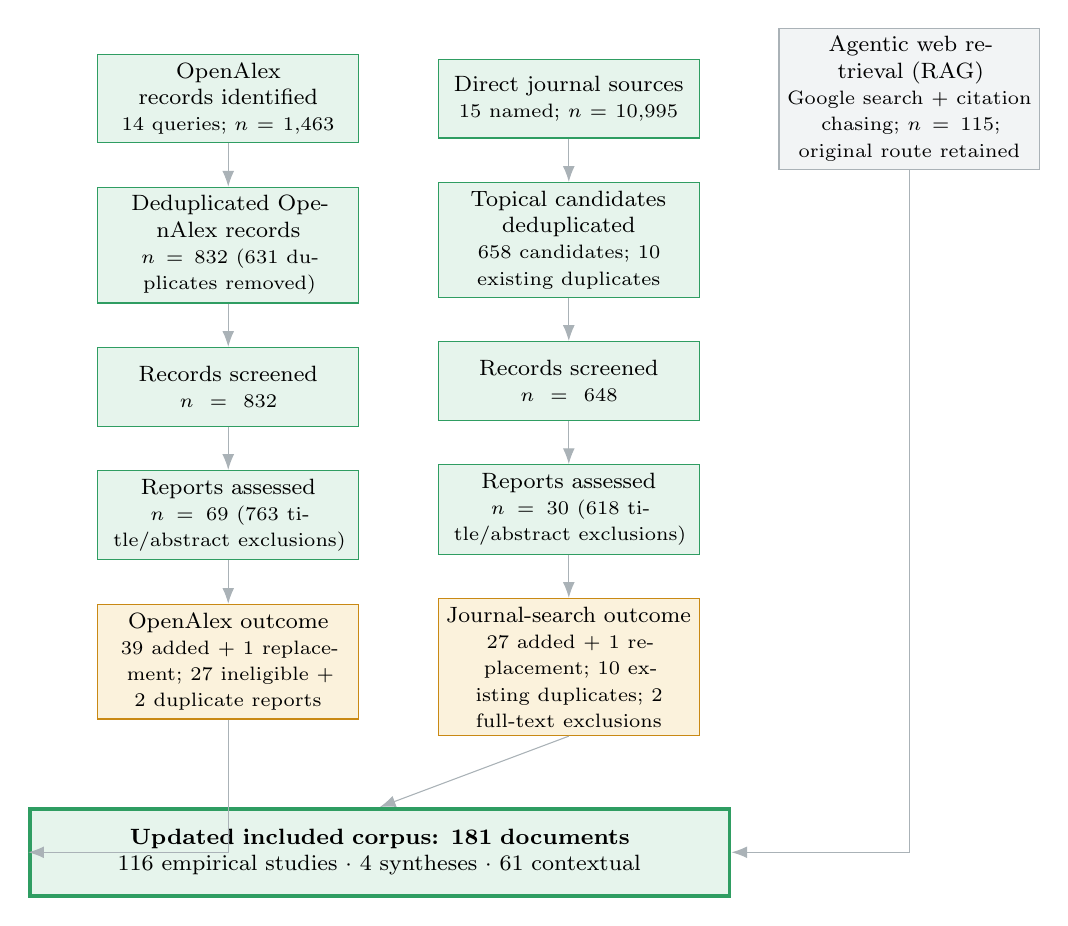
\begin{tikzpicture}[
  font=\footnotesize,
  box/.style={draw, align=center, minimum height=1.0cm, inner sep=3pt, text width=3.1cm},
  outbox/.style={draw=neutralline, fill=neutralbox, align=center, minimum height=1.0cm, inner sep=3pt, text width=3.1cm},
  finalbox/.style={draw=hiw, line width=1.4pt, fill=implbox, align=center, minimum height=1.1cm, inner sep=4pt, text width=8.6cm},
  >={Latex[length=2mm]}
]
\node[box, fill=implbox, draw=hiw] (oa1) {OpenAlex records identified\\\scriptsize 14 queries; $n=1{,}463$};
\node[box, fill=implbox, draw=hiw, below=0.55cm of oa1] (oa2) {Deduplicated OpenAlex records\\\scriptsize $n=832$ (631 duplicates removed)};
\node[box, fill=implbox, draw=hiw, below=0.55cm of oa2] (oa3) {Records screened\\\scriptsize $n=832$};
\node[box, fill=implbox, draw=hiw, below=0.55cm of oa3] (oa4) {Reports assessed\\\scriptsize $n=69$ (763 title/abstract exclusions)};
\node[box, fill=verifybox, draw=modw, below=0.55cm of oa4] (oa5) {OpenAlex outcome\\\scriptsize 39 added + 1 replacement; 27 ineligible + 2 duplicate reports};

\node[box, fill=implbox, draw=hiw, right=1.0cm of oa1] (j1) {Direct journal sources\\\scriptsize 15 named; $n=10{,}995$};
\node[box, fill=implbox, draw=hiw, below=0.55cm of j1] (j2) {Topical candidates deduplicated\\\scriptsize 658 candidates; 10 existing duplicates};
\node[box, fill=implbox, draw=hiw, below=0.55cm of j2] (j3) {Records screened\\\scriptsize $n=648$};
\node[box, fill=implbox, draw=hiw, below=0.55cm of j3] (j4) {Reports assessed\\\scriptsize $n=30$ (618 title/abstract exclusions)};
\node[box, fill=verifybox, draw=modw, below=0.55cm of j4] (j5) {Journal-search outcome\\\scriptsize 27 added + 1 replacement; 10 existing duplicates; 2 full-text exclusions};

\node[outbox, right=1.0cm of j1] (rag) {Agentic web retrieval (RAG)\\\scriptsize Google search + citation chasing; $n=115$; original route retained};

\node[finalbox, below=0.9cm of j5, xshift=-2.4cm] (final) {\textbf{Updated included corpus: 181 documents}\\116 empirical studies $\cdot$ 4 syntheses $\cdot$ 61 contextual};

\draw[->, neutralline] (oa1) -- (oa2);
\draw[->, neutralline] (oa2) -- (oa3);
\draw[->, neutralline] (oa3) -- (oa4);
\draw[->, neutralline] (oa4) -- (oa5);
\draw[->, neutralline] (j1) -- (j2);
\draw[->, neutralline] (j2) -- (j3);
\draw[->, neutralline] (j3) -- (j4);
\draw[->, neutralline] (j4) -- (j5);
\draw[->, neutralline] (oa5.south) |- (final.west);
\draw[->, neutralline] (j5.south) -- (final.north);
\draw[->, neutralline] (rag.south) |- (final.east);
\end{tikzpicture}
\caption{PRISMA-style flow of records through the updated review. The review combines 115 documents from agentic web retrieval, 39 documents added through OpenAlex and 27 documents added by direct searches of 15 software-engineering journals. The journal search enumerated 10,995 records, retained 658 topical candidates, found 10 existing-corpus duplicates, screened or reassessed 648 records and assessed 30 reports. Seventeen empirical studies, two syntheses and eight contextual documents were added, and one synthesis was replaced by its peer-reviewed version. The OpenAlex update ran on 29 July 2026 and the direct journal search on 31 July 2026.}
\label{fig:prisma}
\end{figure}

\paragraph{2. What did the risk-of-bias assessment find?}
\label{sec:risk-of-bias}
Risk of bias tests whether a study's design could systematically overstate or understate its result. It does not measure the size, relevance or practical usefulness of the finding. A large observational study may therefore provide useful scenario evidence even when it cannot establish that AI caused the reported effect.

The clearest causal evidence came from randomised trials. Most release-level and agent-native findings came from non-randomised studies, cases or benchmarks, where team differences, adoption choices and concurrent workflow changes could explain part of the result.

\begin{table}[htbp]
\centering
\caption{Risk-of-bias judgements by study design.}
\label{tab:rob}
\small
\begin{tabular}{@{}p{3.6cm}rp{3.4cm}p{5.3cm}@{}}
\toprule
\textbf{Study design} & \textbf{Studies} & \textbf{Risk judgements} & \textbf{What this means} \\
\midrule
Randomised trials & 10 & 9 some concerns; 1 high & Best causal evidence, with some reporting or adherence limitations \\
Non-randomised interventions & 18 & 2 moderate; 16 serious & Other differences between adopters and controls may explain part of the effect \\
Quasi-experiments & 18 & 13 some concerns; 5 high & Comparison groups were not always equivalent \\
Observational studies & 39 & 28 some concerns; 11 high & Useful for associations, but not isolated causal effects \\
Cases and benchmarks & 31 & 15 some concerns; 16 high & Useful for showing possibilities and failure modes, not expected gains \\
\bottomrule
\end{tabular}
\end{table}

None met the strict low-risk standard across every applicable domain. This does not make the evidence unusable; it means precise causal claims require caution. Randomised studies were assessed with RoB~2 \citep{methodrob2}, non-randomised interventions with ROBINS-I~V2 \citep{methodrobinsi}, and other designs with JBI tools \citep{methodjbi}. The 116 study-level assessments, summary and decision rules are published with the review at \url{https://reinvently.co.uk/research/ai-coding-productivity/risk-of-bias/}.

\paragraph{3. How was each study weighted?}
\label{sec:evidence-appraisal}
Each of the \textbf{116 empirical studies} received an evidence-weight grade. This incorporated the risk-of-bias judgement and also considered whether the outcome directly answered the review question, how precisely it was measured and how relevant the workflow was to real software delivery.

\begin{table}[htbp]
\centering
\caption{Evidence-weight grades across the 116 included empirical studies.}
\label{tab:evidence-weight}
\small
\begin{tabular}{@{}lrp{9.5cm}@{}}
\toprule
\textbf{Evidence weight} & \textbf{Included studies} & \textbf{Interpretation} \\
\midrule
\textcolor{hiw}{\textbf{High}} & 12 & Credible comparator, sufficiently direct outcome and no identified material limitation likely to reverse the result \\
\textcolor{modw}{\textbf{Moderate}} & 77 & Useful comparative or directly measured evidence with residual bias, confounding, indirectness or precision limitations \\
\textcolor{loww}{\textbf{Low}} & 27 & Small or weakly controlled study, historical baseline, self-report, organisational case or counterfactual estimate \\
\bottomrule
\end{tabular}
\end{table}

Contextual documents and secondary syntheses were not graded as primary evidence. The studies were too different for a meaningful pooled estimate, so findings were grouped by degree of automation and delivery stage. Causal claims were limited to credible comparisons; telemetry and case estimates were treated as associations. Every productivity conclusion can be traced from its effect estimate (\texttt{E}) to its study (\texttt{ST}) and source. The study-level evidence-weight register publishes one grade for each of the 116 empirical studies, including all 72 adjacent-outcome studies. The separate operating-model audit retains the effect-level grades and plotting decisions for the 46 productivity estimates. Both are published at \url{https://reinvently.co.uk/research/ai-coding-productivity/}.

\paragraph{4. What survived the sensitivity analysis?}
\label{sec:sensitivity-analysis}
\begin{finding}
Removing results with serious or high risk of bias still leaves bounded assistant studies pointing to gains of roughly \textbf{20--30\%}. It leaves insufficient evidence for a precise release multiplier or a causal \textbf{4.5$\times$} agent-native gain. The \textbf{1.2$\times$} and \textbf{4.5$\times$} figures are therefore planning scenarios, not expected effects.
\end{finding}

\section{Results: How do reported gains vary by degree of automation?}
\label{sec:results}
The findings are grouped by the three operating models defined in the abstract, each representing a different degree of automation. A separate downstream-conversion section then tests how gains in coding activity survive into releases and actual use.

\begin{figure}[htbp]
\centering
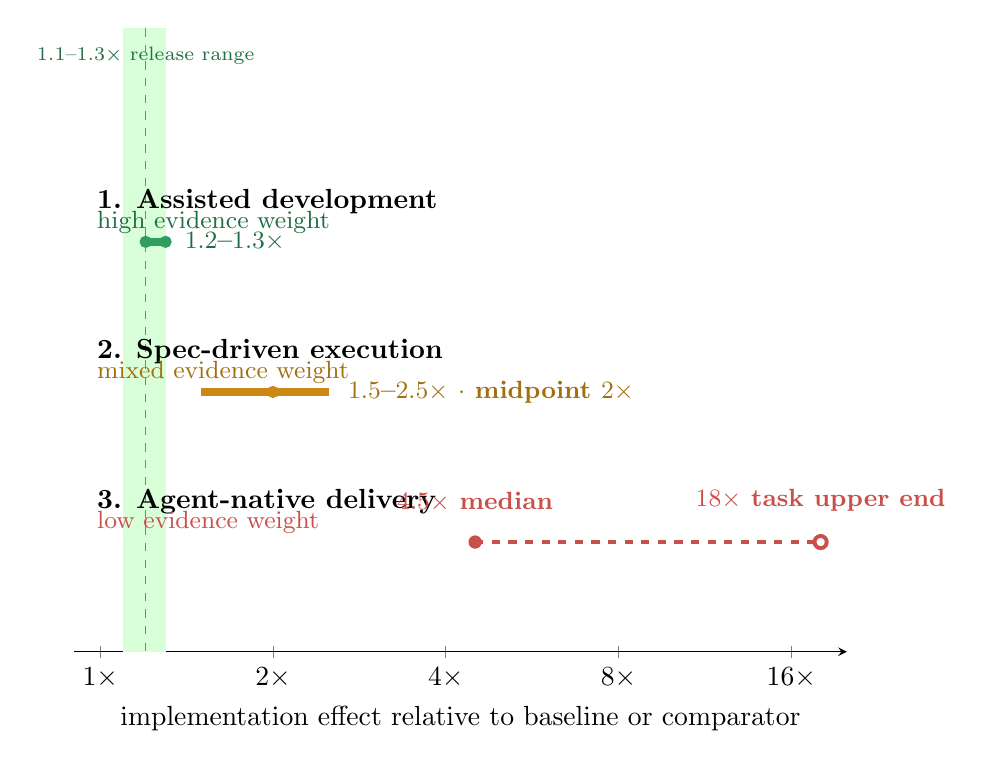
\begin{tikzpicture}
\begin{semilogxaxis}[
  width=0.94\linewidth, height=9.5cm,
  xmin=0.9, xmax=20,
  xtick={1,2,4,8,16},
  xticklabels={$1\times$,$2\times$,$4\times$,$8\times$,$16\times$},
  xlabel={implementation effect relative to baseline or comparator},
  ymin=-0.55, ymax=4.85,
  y dir=reverse,
  ytick=\empty,
  axis y line=none,
  axis x line=bottom,
  clip=false,
]
\draw[green!15,fill=green!15] (axis cs:1.1,-0.55) rectangle (axis cs:1.3,4.85);
\node[anchor=south, font=\scriptsize, text=hiw!70!black] at (axis cs:1.2,-0.15) {$1.1$--$1.3\times$ release range};
\draw[gray, dashed] (axis cs:1.2,-0.55) -- (axis cs:1.2,4.85);

\node[anchor=west, font=\bfseries] at (axis cs:0.95,0.95) {1. Assisted development};
\node[anchor=west, font=\small, text=hiw!70!black] at (axis cs:0.95,1.13) {high evidence weight};
\draw[hiw, line width=3pt] (axis cs:1.2,1.3) -- (axis cs:1.3,1.3);
\filldraw[hiw] (axis cs:1.2,1.3) circle (2pt);
\filldraw[hiw] (axis cs:1.3,1.3) circle (2pt);
\node[anchor=west, font=\small\bfseries, text=hiw!70!black] at (axis cs:1.35,1.3) {$1.2$--$1.3\times$};

\node[anchor=west, font=\bfseries] at (axis cs:0.95,2.25) {2. Spec-driven execution};
\node[anchor=west, font=\small, text=modw!80!black] at (axis cs:0.95,2.43) {mixed evidence weight};
\draw[modw, line width=3pt] (axis cs:1.5,2.6) -- (axis cs:2.5,2.6);
\filldraw[modw] (axis cs:2.0,2.6) circle (2pt);
\node[anchor=west, font=\small\bfseries, text=modw!80!black] at (axis cs:2.6,2.6) {$1.5$--$2.5\times$ $\cdot$ midpoint $2\times$};

\node[anchor=west, font=\bfseries] at (axis cs:0.95,3.55) {3. Agent-native delivery};
\node[anchor=west, font=\small, text=loww] at (axis cs:0.95,3.73) {low evidence weight};
\draw[loww, dashed, line width=1.6pt] (axis cs:4.5,3.9) -- (axis cs:18,3.9);
\filldraw[loww] (axis cs:4.5,3.9) circle (2.2pt);
\draw[loww, fill=white, line width=1.4pt] (axis cs:18,3.9) circle (2.2pt);
\node[anchor=south, font=\small\bfseries, text=loww] at (axis cs:4.5,3.72) {$4.5\times$ median};
\node[anchor=south, font=\small\bfseries, text=loww] at (axis cs:18,3.72) {$18\times$ task upper end};
\end{semilogxaxis}
\end{tikzpicture}
\caption{Implementation-stage planning ranges at three levels of AI autonomy, on a logarithmic scale. Assisted development has a planning range of 1.2 to 1.3 times and high evidence weight. Spec-driven execution has a 1.5 to 2.5 times range and mixed evidence weight. Agent-native delivery has a low-weight case median of 4.5 times, with an 18 times task-specific upper-end case. A green band marks the 1.1 to 1.3 times release-output range. These are implementation-stage planning ranges, not release forecasts or pooled effects. Assisted development is supported by controlled studies. The Level 2 range combines bounded comparisons and organisational cases. The Level 3 median and 18$\times$ upper end come from low-weight organisational estimates using different tasks and baselines. The shaded band shows the separate 10--30\% release-output range observed across tool generations in the largest matched event study.}
\label{fig:ladder}
\end{figure}

\subsection{Assisted development: task completion and local output}
\label{sec:task-results}
The strongest evidence concerns assistants operating inside otherwise conventional human-led workflows. The measured effects are heterogeneous, and tool choice changes the interaction model without determining the outcome by itself.

A randomised trial involving 96 Google engineers found that AI assistance reduced time on a complex enterprise task by an estimated 21\%, although the confidence interval was wide \citep{st01}. Three field experiments at Microsoft, Accenture and a Fortune 100 company covered 4,867 developers and found a 26.08\% increase in completed tasks \citep{st02}.

A 109-participant controlled experiment found that ChatGPT helped with simple coding puzzles but did not improve efficiency or quality on a more typical software-development task \citep{st03}. A later controlled study of 69 participants found no strong overall time effect, but AI users achieved more than twice the median task completeness \citep{st08} and scored 12.5\% lower on code-ownership questions. Together these results show why task completion, time and understanding should be reported separately.

\begin{finding}
\textbf{Bottom line:} multiple controlled studies support an assisted-development reference value near \textbf{1.25$\times$}, but the effect varies by task, repository familiarity and developer experience. The range includes null results and a 19\% slowdown. This is the strongest of the three evidence tiers.
\end{finding}

\paragraph{Extended assisted-development evidence.}
Two smaller crossover experiments add qualified positive evidence. In a 32-person ICSE study, an in-IDE code-understanding assistant helped participants complete 0.47 more subtasks than web search \citep{st09}, but did not significantly change completion time or comprehension. An 18-person JavaScript study found that participants using ClueBot finished faster and made fewer errors \citep{st10}; its small student-heavy sample and high risk of bias limit generalisation.

The updated search adds two comparative task studies without changing that conclusion. In a 27-student controlled study, three completion tools reduced average recorded time by 11--14\% \citep{st86}, but only two of the seven participants who finished both assigned tasks were faster with AI. A quasi-experiment found that some non-programmers using ChatGPT completed small, well-specified tasks faster than programmers without AI, but the design lacked both a programmers-with-AI group and a non-programmers-without-AI group \citep{st70}.

A larger preregistered maintainability experiment also captured an assisted-development speed result. In its first phase, participants who chose an AI assistant completed a Java feature task in 30.7\% less median time \citep{st27}. The comparison was observational rather than randomised, but the study explicitly predates autonomous coding agents and therefore belongs at Level 1.

A larger quasi-experiment at Ant Group compared matched teams during the staged introduction of CodeFuse. Across a sample of 1,219 programmers, code output increased by 55\% \citep{st18}. More conservative specifications found gains of roughly 13--22\% in tasks completed and related workflow measures. Effects were concentrated among junior developers, and lines of code remained the principal outcome.

A public-sector study by GovTech Singapore reported 21--28\% faster coding and task completion with GitHub Copilot \citep{st28}. The direction is consistent with the larger controlled studies, although the disclosed design provides less protection against selection and reporting effects.

A separate Anthropic randomised trial found only a small, statistically non-significant task-speed improvement, while participants using AI scored 17 percentage points lower on a subsequent mastery test (50\% against 67\%) \citep{st56}. This does not establish a long-term productivity loss, but it identifies skill retention as an omitted outcome in most speed studies.

Enterprise studies based mainly on self-report provide useful triangulation but weaker effect estimates. An IBM study of 669 developers found heterogeneous perceived productivity effects from watsonx Code Assistant \citep{st57}, while a Microsoft randomised diary study found that 84\% reported positive changes in daily work practices \citep{st58} without a corresponding change in trust in generated code.

Interaction studies expose work that completion metrics miss: prompting, inspecting, editing and recovering from suggestions. Microsoft's CUPS study of 21 programmers made those costs observable \citep{st59}. A randomised study of proactive programming assistance found benefits but strong interface effects \citep{ctx33}. A five-day professional field study similarly found that poorly timed proactive assistance could interrupt flow (ProAIDE) \citep{ctx17}. Across 66,239 industrial interactions, accepted suggestions differed systematically by developer history, project history and code context; a predictive filter reduced likely interruptions, but did not estimate delivery speed \citep{st96}.

New journal evidence reinforces that interaction design changes outcomes without supplying an end-to-end multiplier. In a data-science user study, naming the current workflow step significantly increased recommendation acceptance, while presenting alternative code paths did not (ST-104) \citep{st104}. A 27-student instrumented study found acceptance varied by task and suggestion type, and that editing existing code often caused backtracking (ST-102) \citep{st102}.

Adoption evidence helps explain these mechanisms but does not establish delivery gains. GitHub's telemetry-linked study of 2,047 respondents associated higher completion acceptance with higher perceived productivity \citep{ctx30}. A peer-reviewed 410-developer usability survey identified fewer keystrokes, faster completion and syntax recall as leading benefits, but control and non-functional requirements as common failures \citep{ctx01}. A 481-programmer journal survey found that 84.2\% used assistants at least occasionally, while inaccurate output, lack of trust and weak project context remained leading barriers \citep{ctx58}. A seven-company European case study found use was still predominantly personal and assistive rather than process-level \citep{ctx46}.

Smaller controlled studies reinforce the importance of task selection. At ANZ Bank, a six-week controlled study reported 42.3\% less completion time on Python exercises \citep{st06}. A 24-person within-subject study found higher requirements completed per minute with both conversational and completion interfaces, although its tasks were short and only nine participants were professionals \citep{st07}.

Industrial completion systems provide credible day-to-day activity measures, although these are not product outcomes. Meta's CodeCompose supplied 8\% of accepted code for 16,000 users \citep{st33}; extending it to multi-line suggestions nearly doubled keystrokes saved from 9\% to 17\% \citep{st23}. The UK Government's trial made 2,500 licences available and combined telemetry with surveys; participants reported approximately one hour saved per working day (56 minutes) \citep{st32}, but the result was self-reported rather than a causal time study.

\subsection{Spec-driven execution: bounded delegation}
\label{sec:specified-results}
At the second level, the engineer defines an outcome, constraints and acceptance checks; the agent performs multi-file implementation; the engineer still reads and owns the change. Evidence here is less controlled because organisations usually adopt several changes at once.

Two bounded comparisons fit this operating model more closely than assisted development. In a 24-developer brownfield-onboarding experiment, Copilot Agent reduced mean completion time by 61.7\% relative to Copilot Ask \citep{st05} and workload by 57.4\%, without a significant correctness improvement; interaction shifted from active collaboration towards passive supervision. In a repeated single-developer comparison, Cursor completed the same defined web app in about 13 minutes with two to three prompts, against 27 minutes and five to six prompts for ChatGPT, but there was no manual baseline \citep{st69}.

A separate controlled comparison found that agents reduced effort and completed some otherwise inaccessible tasks, but did not remove the developer's need to understand and verify their behaviour \citep{ctx13}. This supports the workflow distinction without supplying a comparable delivery multiplier.

\paragraph{Extended spec-driven evidence.}
A peer-reviewed test-driven workflow supplies direct evidence for specification as a verification aid. In a 15-programmer study, TiCoder used generated tests to clarify intent; participants were significantly more likely to evaluate generated code correctly and reported lower task-induced cognitive load (ST-111) \citep{st111}. The accompanying model benchmark improved code-generation accuracy, but the human study did not estimate delivery throughput.

An Amazon Prime Video Financial Systems team provides a more specific example. A senior engineer spent three weeks decomposing work and writing detailed requirements before a ten-day sprint. The team used spec-driven development for complex features and direct agent assistance where requirements were already clear. It reduced a 90-week estimate to 24 weeks---approximately 3.75$\times$ acceleration, which AWS rounds to 4$\times$---and produced 556 commits against a baseline of 96, nearly six times the usual output \citep{st31}.

The study conditions limit external validity: six engineers had no on-call work, no other projects, minimal meetings and no context switching. Specification was part of the system, not the only intervention.

Cisco reports teams achieving up to 3$\times$ productivity in technical-debt workflows \citep{st38}. Its agent investigates a quality issue, produces a written plan, implements in a fresh session and opens a pull request for human review. The work is unusually deterministic, with SonarQube providing a ready-made issue description and verification layer.

Amazon reports a broader but similarly bounded transformation programme. Developers review and refine Amazon Q Developer's plan before its transformation agent implements multi-step upgrades. Across tens of thousands of production Java applications, Amazon estimates that this saved 4,500 developer-years \citep{st40}. The estimate derives from migrated dependencies and assumed manual effort rather than a concurrent control group, so it demonstrates scale rather than a transferable acceleration factor.

Evidence on specification quality shows why ``more detail'' is not sufficient by itself. Copilot generated both repayments and reproductions of technical debt when prompted with 1,140 variants derived from TODO comments \citep{ctx08}. By contrast, Meta found that pre-computing context across 4,100 files reduced agent tool calls by 40\% \citep{ctx25}, while a separate internal agent reduced approximately ten hours of performance-regression investigation to 30 minutes \citep{ctx26}. These first-party cases suggest that explicit context and executable feedback reduce search cost; they do not isolate specification as a causal multiplier.

Specification also cannot recover business knowledge that was never made explicit. In a controlled .NET study, an agent could produce technically valid changes while violating intended behaviour when historical terminology and business rules were ambiguous \citep{st75}. An end-to-end meeting-to-pull-request pipeline performed reliably on individual issues, but 44 workflow runs exposed different conflict modes when agents operated in parallel on sparse and structured repositories \citep{st81}. Strong specifications therefore need explicit domain definitions, repository contracts and conflict handling---not task prose alone.

A peer-reviewed ICSE 2026 study examined an expert-led, AI-implemented workflow on PicoScenes, a 1.52-million-line industrial system with a ten-year history. The authors report 68.3\% less feature-implementation time \citep{st21}, alongside 28.2\% lower mean cyclomatic complexity and 50\% fewer defects. The comparison concerns one system and a bundled development method, but it provides unusually detailed evidence that specified delegation can extend beyond small greenfield tasks.

Anthropic's internal mixed-methods study offers a second organisational data point. Engineers self-reported a 50\% average productivity gain as Claude use expanded, while internal telemetry showed a 67\% increase in merged pull requests per engineer per day \citep{st30}. The before-and-after design cannot isolate Claude from team growth, task selection or workflow change.

\begin{finding}
\textbf{Review finding:} reported outcomes support a \textbf{1.5--2.5$\times$ planning range} for bounded spec-driven execution with human review. The \textbf{2$\times$} midpoint is not a pooled effect: one small controlled agent-versus-assistant comparison implies 2.61$\times$ potential throughput, while the remaining evidence is heterogeneous and mainly case-based. \textbf{Basis:} E-05, E-21, E-30, E-38, E-39, E-42, E-43.
\end{finding}

\subsection{Agent-native delivery: production cases}
\label{sec:agent-native-results}
The largest claims concern teams that restructure repositories, planning, testing, review and parallel execution so agents can operate for longer with less synchronous human attention.

Salesforce reports that autonomous tools now write code, review pull requests, generate tests and drive deployments across its engineering organisation. Work items completed per developer rose 50.8\% year over year, while its ``Effective Output'' measure rose 151.3\% \citep{st29}. The organisation also standardised on Claude Code, removed token limits and rebuilt workflows, so the result is an agent-native organisational bundle rather than an isolated tool effect.

AWS studied more than 50 teams and found that the 25 combining new tools with new practices outperformed those that simply added AI to existing workflows. In separate Amazon Stores pilots---typical teams working their regular backlogs, with no special conditions or handpicked engineers---the median productivity gain was 4.5$\times$ \citep{st31}, with some teams exceeding 10$\times$ normalised deployment velocity. Its Bedrock pathfinder reported 20$\times$ normalised commit velocity, but this involved six senior engineers rebuilding an inference engine against a 30-developer, 12-to-18-month estimate under highly unusual conditions. Deployment velocity is the more useful number.

OpenAI describes an internal product built with no manually written code: approximately one million lines and 1,500 merged pull requests directed initially by three engineers over five months. The team estimates it took one-tenth of the manual development time \citep{st39}. This is a serious production account with active users, but the 10$\times$ figure remains the team's counterfactual estimate rather than an experiment.

Salesforce reports a 33-endpoint migration completed in 13 days rather than an estimated 231 person-days---an 18$\times$ task-specific acceleration \citep{st29}. It used reference implementations, reusable rules, isolated environments and autonomous build-fix-validate loops. Migration work is repetitive and parallelisable, limiting the result's generalisability to novel product development.

\paragraph{Extended agent-native evidence.}
Usage telemetry also shows that agentic work remains strongly shaped by human expertise. Anthropic's analysis of approximately 400,000 Claude Code sessions found that people made most planning decisions while the agent made most execution decisions; greater domain expertise was associated with a higher probability of verifiable success \citep{ctx03}.

Repository evidence shows broad adoption without establishing productivity. A study of 128,018 GitHub projects estimated coding-agent adoption at 22.20--28.66\% by February 2026 and found that agent-assisted commits were larger than human-only commits \citep{st63}. Across 26,760 agent-authored pull requests, agents imported libraries in 29.5\% of changes but introduced new dependencies in only 1.3\%; 75\% of those additions specified a version \citep{st61}. These traces establish that agents participate in real repository work, but larger changes and dependency interactions also expand the integration surface.

Agent benchmarks define a capability ceiling rather than a workplace-productivity effect. SWE-Lancer maps more than 1,400 real freelance tasks to approximately \$1 million of historical payouts \citep{ctx27}. The ICLR 2024 SWE-bench study \citep{ctx51} and SWE-agent \citep{ctx48} show that repository tools and execution feedback can materially improve issue resolution. SWE-bench Multimodal exposes weaker performance on visual JavaScript tasks \citep{ctx50}, while GitTaskBench adds workflow-driven repository use and an economic metric \citep{ctx23}. The paired SWE-Skills-Bench result is a useful constraint: 39 of 49 packaged skills produced no pass-rate gain and average improvement was only 1.2\% \citep{ctx52}. None of these results can be converted directly into hours saved without a human workflow comparator.

\begin{finding}
\textbf{Review finding:} reported agent-native workflows cluster around \textbf{2.5--10$\times$}, with a higher task-specific migration estimate. AWS's \textbf{4.5$\times$ median} is the most suitable central reference in the available case evidence. Evidence weight remains low because the studies are observational, heterogeneous and frequently vendor-published. \textbf{Basis:} E-29, E-31, E-40, E-41.
\end{finding}

\subsection{Study results by operating model and exposure}
\label{sec:study-plot}
The evidence changes in both magnitude and strength across the three operating models. Figure~\ref{fig:scatter} represents all 34 estimates that can be expressed numerically against a baseline or comparator. Studies were assigned by their observed workflow, not the product name; the 46-estimate classification audit records each decision (published at \url{https://reinvently.co.uk/research/ai-coding-productivity/operating-model-audit.csv}). Seven estimates aggregate several modes or do not disclose enough workflow detail, so they appear in a separate cross-level group rather than being forced into an automation tier. E-11 appears at all three levels because it reports separate release effects for autocomplete, interactive agents and autonomous agents. Twelve other productivity estimates report directional, absolute or otherwise non-comparable outcomes. Where a study reports time saved, the value is converted to potential throughput using the reciprocal relationship defined in Section~\ref{sec:outcome-definitions}. The values remain heterogeneous and are not pooled.

\begin{figure}[p]
\centering
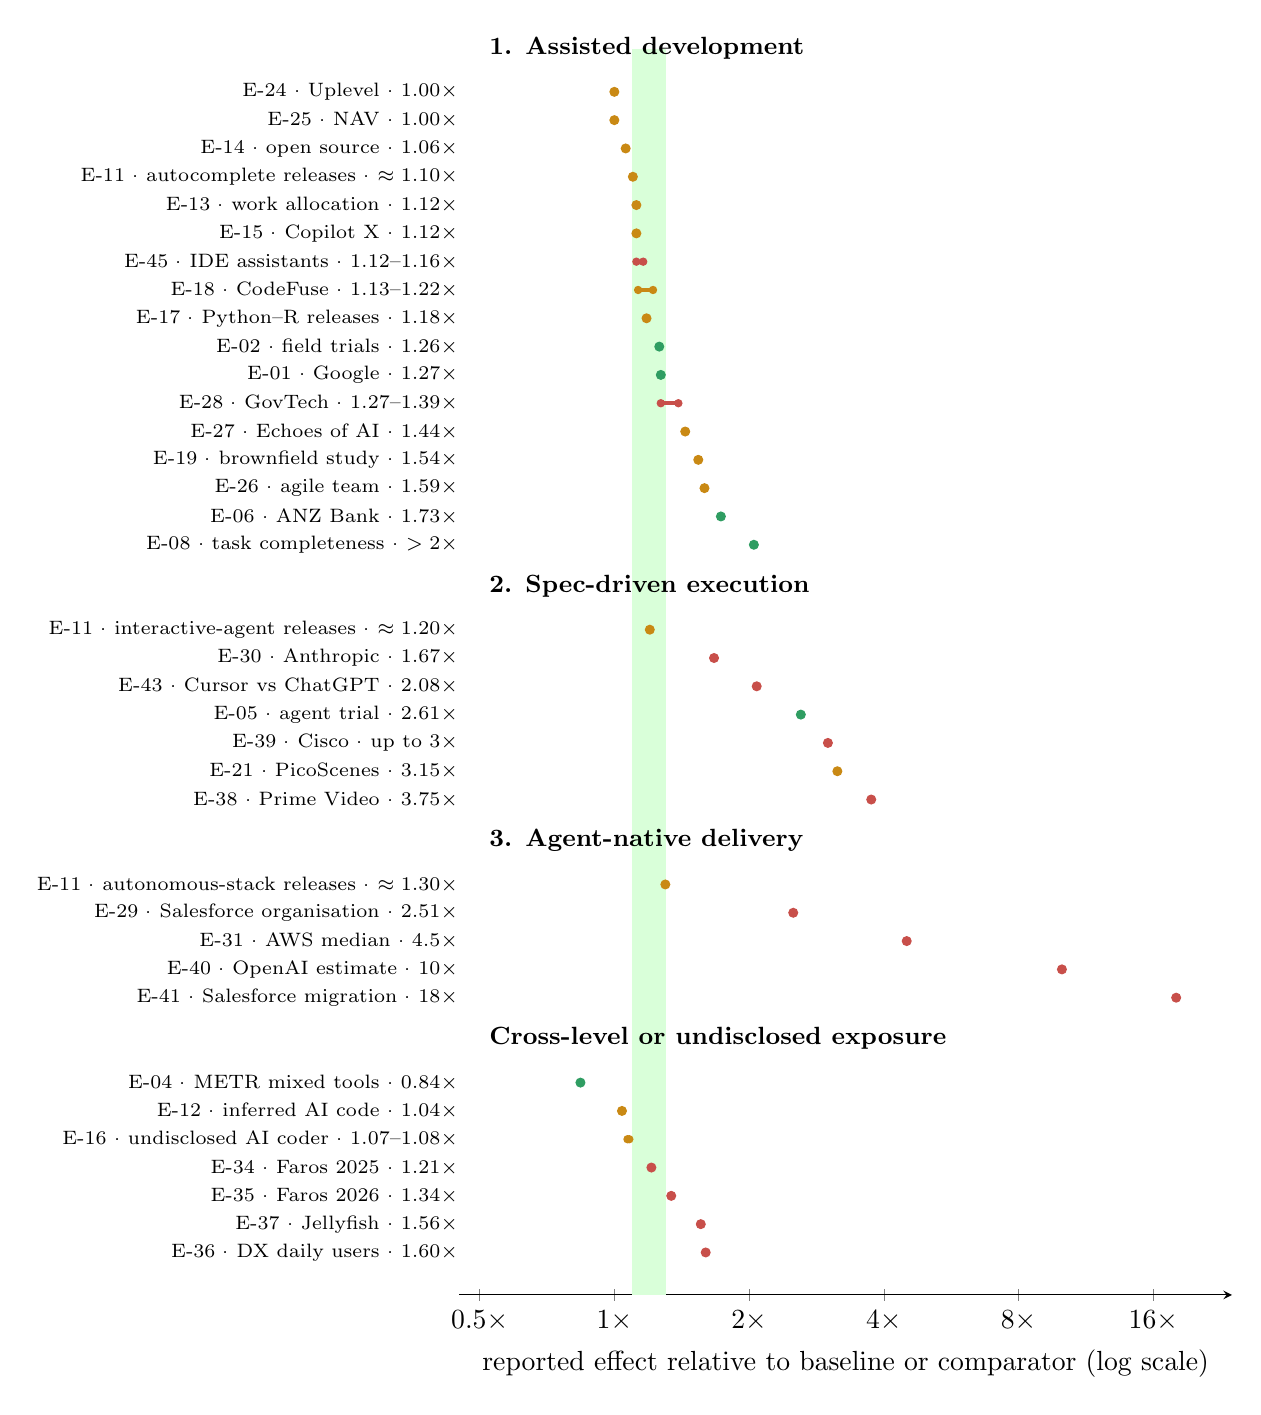
\begin{tikzpicture}
\begin{semilogxaxis}[
  width=0.94\linewidth, height=17.4cm,
  xmin=0.45, xmax=24,
  xtick={0.5,1,2,4,8,16},
  xticklabels={$0.5\times$,$1\times$,$2\times$,$4\times$,$8\times$,$16\times$},
  xlabel={reported effect relative to baseline or comparator (log scale)},
  ymin=-43.5, ymax=0.5,
  ytick=\empty,
  axis y line=none,
  axis x line=bottom,
  clip=false,
]
\draw[green!15,fill=green!15] (axis cs:1.1,-43.5) rectangle (axis cs:1.3,0.5);
%% AUTO-GENERATED forest-plot body -- see scratchpad/gen_fig2.py; 36 point-rows for 34 distinct estimates (E-11 plotted three times).
\node[anchor=west, font=\bfseries\small] at (axis cs:0.5,0.55) {1. Assisted development};
\node[anchor=west, font=\bfseries\small] at (axis cs:0.5,-18.45) {2. Spec-driven execution};
\node[anchor=west, font=\bfseries\small] at (axis cs:0.5,-27.45) {3. Agent-native delivery};
\node[anchor=west, font=\bfseries\small] at (axis cs:0.5,-34.45) {Cross-level or undisclosed exposure};
\node[anchor=east, font=\scriptsize] at (axis cs:0.47,-1) {E-24 \textperiodcentered\ Uplevel \textperiodcentered\ $1.00\times$};
\filldraw[modw] (axis cs:1.0,-1) circle (1.6pt);
\node[anchor=east, font=\scriptsize] at (axis cs:0.47,-2) {E-25 \textperiodcentered\ NAV \textperiodcentered\ $1.00\times$};
\filldraw[modw] (axis cs:1.0,-2) circle (1.6pt);
\node[anchor=east, font=\scriptsize] at (axis cs:0.47,-3) {E-14 \textperiodcentered\ open source \textperiodcentered\ $1.06\times$};
\filldraw[modw] (axis cs:1.06,-3) circle (1.6pt);
\node[anchor=east, font=\scriptsize] at (axis cs:0.47,-4) {E-11 \textperiodcentered\ autocomplete releases \textperiodcentered\ $\approx1.10\times$};
\filldraw[modw] (axis cs:1.1,-4) circle (1.6pt);
\node[anchor=east, font=\scriptsize] at (axis cs:0.47,-5) {E-13 \textperiodcentered\ work allocation \textperiodcentered\ $1.12\times$};
\filldraw[modw] (axis cs:1.12,-5) circle (1.6pt);
\node[anchor=east, font=\scriptsize] at (axis cs:0.47,-6) {E-15 \textperiodcentered\ Copilot X \textperiodcentered\ $1.12\times$};
\filldraw[modw] (axis cs:1.12,-6) circle (1.6pt);
\node[anchor=east, font=\scriptsize] at (axis cs:0.47,-7) {E-45 \textperiodcentered\ IDE assistants \textperiodcentered\ $1.12$--$1.16\times$};
\draw[loww, line width=1.4pt] (axis cs:1.12,-7) -- (axis cs:1.16,-7);
\filldraw[loww] (axis cs:1.12,-7) circle (1.3pt);
\filldraw[loww] (axis cs:1.16,-7) circle (1.3pt);
\node[anchor=east, font=\scriptsize] at (axis cs:0.47,-8) {E-18 \textperiodcentered\ CodeFuse \textperiodcentered\ $1.13$--$1.22\times$};
\draw[modw, line width=1.4pt] (axis cs:1.13,-8) -- (axis cs:1.22,-8);
\filldraw[modw] (axis cs:1.13,-8) circle (1.3pt);
\filldraw[modw] (axis cs:1.22,-8) circle (1.3pt);
\node[anchor=east, font=\scriptsize] at (axis cs:0.47,-9) {E-17 \textperiodcentered\ Python--R releases \textperiodcentered\ $1.18\times$};
\filldraw[modw] (axis cs:1.18,-9) circle (1.6pt);
\node[anchor=east, font=\scriptsize] at (axis cs:0.47,-10) {E-02 \textperiodcentered\ field trials \textperiodcentered\ $1.26\times$};
\filldraw[hiw] (axis cs:1.26,-10) circle (1.6pt);
\node[anchor=east, font=\scriptsize] at (axis cs:0.47,-11) {E-01 \textperiodcentered\ Google \textperiodcentered\ $1.27\times$};
\filldraw[hiw] (axis cs:1.27,-11) circle (1.6pt);
\node[anchor=east, font=\scriptsize] at (axis cs:0.47,-12) {E-28 \textperiodcentered\ GovTech \textperiodcentered\ $1.27$--$1.39\times$};
\draw[loww, line width=1.4pt] (axis cs:1.27,-12) -- (axis cs:1.39,-12);
\filldraw[loww] (axis cs:1.27,-12) circle (1.3pt);
\filldraw[loww] (axis cs:1.39,-12) circle (1.3pt);
\node[anchor=east, font=\scriptsize] at (axis cs:0.47,-13) {E-27 \textperiodcentered\ Echoes of AI \textperiodcentered\ $1.44\times$};
\filldraw[modw] (axis cs:1.44,-13) circle (1.6pt);
\node[anchor=east, font=\scriptsize] at (axis cs:0.47,-14) {E-19 \textperiodcentered\ brownfield study \textperiodcentered\ $1.54\times$};
\filldraw[modw] (axis cs:1.54,-14) circle (1.6pt);
\node[anchor=east, font=\scriptsize] at (axis cs:0.47,-15) {E-26 \textperiodcentered\ agile team \textperiodcentered\ $1.59\times$};
\filldraw[modw] (axis cs:1.59,-15) circle (1.6pt);
\node[anchor=east, font=\scriptsize] at (axis cs:0.47,-16) {E-06 \textperiodcentered\ ANZ Bank \textperiodcentered\ $1.73\times$};
\filldraw[hiw] (axis cs:1.73,-16) circle (1.6pt);
\node[anchor=east, font=\scriptsize] at (axis cs:0.47,-17) {E-08 \textperiodcentered\ task completeness \textperiodcentered\ $>2\times$};
\filldraw[hiw] (axis cs:2.05,-17) circle (1.6pt);
\node[anchor=east, font=\scriptsize] at (axis cs:0.47,-20) {E-11 \textperiodcentered\ interactive-agent releases \textperiodcentered\ $\approx1.20\times$};
\filldraw[modw] (axis cs:1.2,-20) circle (1.6pt);
\node[anchor=east, font=\scriptsize] at (axis cs:0.47,-21) {E-30 \textperiodcentered\ Anthropic \textperiodcentered\ $1.67\times$};
\filldraw[loww] (axis cs:1.67,-21) circle (1.6pt);
\node[anchor=east, font=\scriptsize] at (axis cs:0.47,-22) {E-43 \textperiodcentered\ Cursor vs ChatGPT \textperiodcentered\ $2.08\times$};
\filldraw[loww] (axis cs:2.08,-22) circle (1.6pt);
\node[anchor=east, font=\scriptsize] at (axis cs:0.47,-23) {E-05 \textperiodcentered\ agent trial \textperiodcentered\ $2.61\times$};
\filldraw[hiw] (axis cs:2.61,-23) circle (1.6pt);
\node[anchor=east, font=\scriptsize] at (axis cs:0.47,-24) {E-39 \textperiodcentered\ Cisco \textperiodcentered\ up to $3\times$};
\filldraw[loww] (axis cs:3.0,-24) circle (1.6pt);
\node[anchor=east, font=\scriptsize] at (axis cs:0.47,-25) {E-21 \textperiodcentered\ PicoScenes \textperiodcentered\ $3.15\times$};
\filldraw[modw] (axis cs:3.15,-25) circle (1.6pt);
\node[anchor=east, font=\scriptsize] at (axis cs:0.47,-26) {E-38 \textperiodcentered\ Prime Video \textperiodcentered\ $3.75\times$};
\filldraw[loww] (axis cs:3.75,-26) circle (1.6pt);
\node[anchor=east, font=\scriptsize] at (axis cs:0.47,-29) {E-11 \textperiodcentered\ autonomous-stack releases \textperiodcentered\ $\approx1.30\times$};
\filldraw[modw] (axis cs:1.3,-29) circle (1.6pt);
\node[anchor=east, font=\scriptsize] at (axis cs:0.47,-30) {E-29 \textperiodcentered\ Salesforce organisation \textperiodcentered\ $2.51\times$};
\filldraw[loww] (axis cs:2.51,-30) circle (1.6pt);
\node[anchor=east, font=\scriptsize] at (axis cs:0.47,-31) {E-31 \textperiodcentered\ AWS median \textperiodcentered\ $4.5\times$};
\filldraw[loww] (axis cs:4.5,-31) circle (1.6pt);
\node[anchor=east, font=\scriptsize] at (axis cs:0.47,-32) {E-40 \textperiodcentered\ OpenAI estimate \textperiodcentered\ $10\times$};
\filldraw[loww] (axis cs:10.0,-32) circle (1.6pt);
\node[anchor=east, font=\scriptsize] at (axis cs:0.47,-33) {E-41 \textperiodcentered\ Salesforce migration \textperiodcentered\ $18\times$};
\filldraw[loww] (axis cs:18.0,-33) circle (1.6pt);
\node[anchor=east, font=\scriptsize] at (axis cs:0.47,-36) {E-04 \textperiodcentered\ METR mixed tools \textperiodcentered\ $0.84\times$};
\filldraw[hiw] (axis cs:0.84,-36) circle (1.6pt);
\node[anchor=east, font=\scriptsize] at (axis cs:0.47,-37) {E-12 \textperiodcentered\ inferred AI code \textperiodcentered\ $1.04\times$};
\filldraw[modw] (axis cs:1.04,-37) circle (1.6pt);
\node[anchor=east, font=\scriptsize] at (axis cs:0.47,-38) {E-16 \textperiodcentered\ undisclosed AI coder \textperiodcentered\ $1.07$--$1.08\times$};
\draw[modw, line width=1.4pt] (axis cs:1.07,-38) -- (axis cs:1.08,-38);
\filldraw[modw] (axis cs:1.07,-38) circle (1.3pt);
\filldraw[modw] (axis cs:1.08,-38) circle (1.3pt);
\node[anchor=east, font=\scriptsize] at (axis cs:0.47,-39) {E-34 \textperiodcentered\ Faros 2025 \textperiodcentered\ $1.21\times$};
\filldraw[loww] (axis cs:1.21,-39) circle (1.6pt);
\node[anchor=east, font=\scriptsize] at (axis cs:0.47,-40) {E-35 \textperiodcentered\ Faros 2026 \textperiodcentered\ $1.34\times$};
\filldraw[loww] (axis cs:1.34,-40) circle (1.6pt);
\node[anchor=east, font=\scriptsize] at (axis cs:0.47,-41) {E-37 \textperiodcentered\ Jellyfish \textperiodcentered\ $1.56\times$};
\filldraw[loww] (axis cs:1.56,-41) circle (1.6pt);
\node[anchor=east, font=\scriptsize] at (axis cs:0.47,-42) {E-36 \textperiodcentered\ DX daily users \textperiodcentered\ $1.60\times$};
\filldraw[loww] (axis cs:1.6,-42) circle (1.6pt);
\end{semilogxaxis}
\end{tikzpicture}
\caption{Thirty-four of the review's 46 productivity effect estimates are represented (36 points, since E-11 is plotted at all three operating-model levels). Assisted development, spec-driven execution and agent-native delivery are followed by a cross-level group for mixed or undisclosed exposure. The horizontal axis is logarithmic. Colour represents evidence weight (\textcolor{hiw}{green = high}, \textcolor{modw}{amber = moderate}, \textcolor{loww}{red = low}). A green vertical band marks the 1.1--1.3$\times$ release-output planning range. Excluding the cross-level E-11, 16 are assisted, six are spec-driven, four are agent-native and seven have mixed or undisclosed exposure. Twelve non-comparable estimates and 72 adjacent-outcome studies are not plotted. Time reductions are converted to potential throughput where appropriate. Measures and reference conditions remain heterogeneous and should be compared within operating models rather than averaged.}
\label{fig:scatter}
\end{figure}

\section{Do coding gains survive into production?}
\label{sec:delivery-results}
This conversion is a cross-level outcome rather than a fourth operating model. At Level 1, local task gains must survive integration and review. Levels 2 and 3 can produce much larger increases in implementation activity, but place correspondingly greater demand on validation, release and adoption capacity.

The largest direct study of that conversion followed more than 100,000 GitHub developers using matched event studies and internal usage telemetry. Autocomplete, interactive agents and autonomous agents were associated with cumulative commit gains of 40\%, 140\% and 180\%, respectively. The final effect was much smaller: the 180\% commit increase became 50\% more projects and 30\% more releases \citep{st11}, while analysis across four application marketplaces found no increase in total usage. This is the clearest evidence that code activity, shipped software and realised value are different outcomes.

\begin{figure}[htbp]
\centering
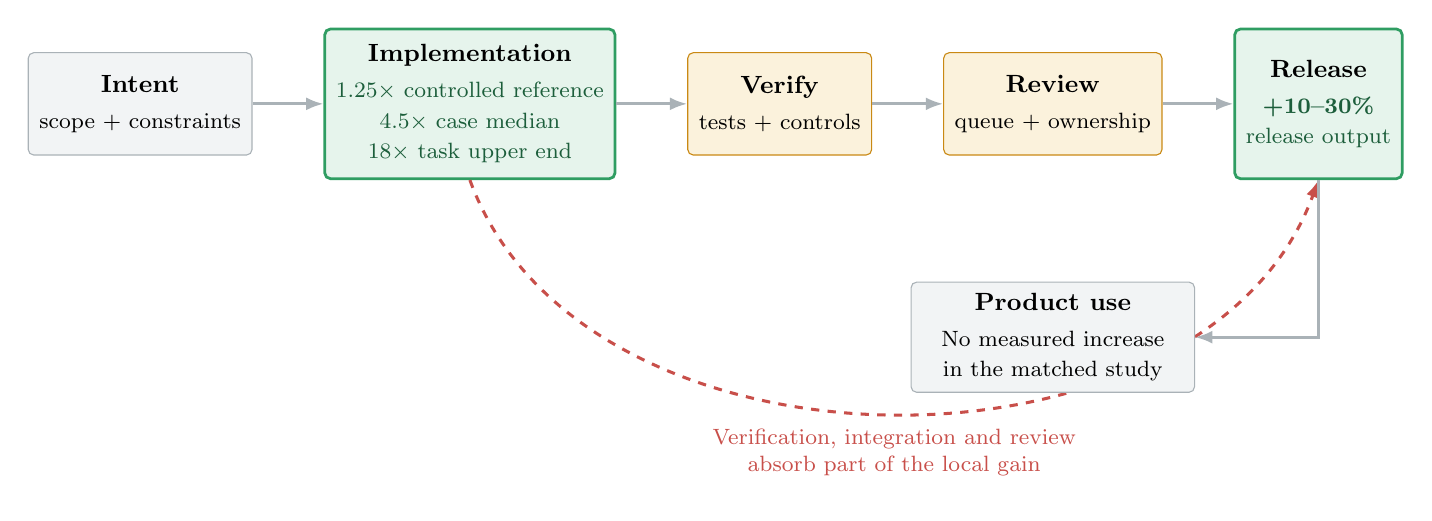
\begin{tikzpicture}[
  font=\small,
  box/.style={draw, rounded corners=2pt, align=center, minimum height=1.3cm, inner sep=4pt},
  >={Latex[length=2.2mm]}
]
\node[box, fill=neutralbox, draw=neutralline, minimum width=2.1cm] (intent) {\textbf{Intent}\\[2pt]\footnotesize scope + constraints};
\node[box, fill=implbox, draw=hiw, line width=1pt, minimum width=2.6cm, minimum height=1.9cm, right=0.9cm of intent] (impl) {\textbf{Implementation}\\[2pt]\footnotesize\textcolor{hiw!60!black}{$1.25\times$ controlled reference}\\\footnotesize\textcolor{hiw!60!black}{$4.5\times$ case median}\\\footnotesize\textcolor{hiw!60!black}{$18\times$ task upper end}};
\node[box, fill=verifybox, draw=modw, minimum width=2.0cm, right=0.9cm of impl] (verify) {\textbf{Verify}\\[2pt]\footnotesize tests + controls};
\node[box, fill=verifybox, draw=modw, minimum width=1.8cm, right=0.9cm of verify] (review) {\textbf{Review}\\[2pt]\footnotesize queue + ownership};
\node[box, fill=implbox, draw=hiw, line width=1pt, minimum width=1.9cm, minimum height=1.9cm, right=0.9cm of review] (release) {\textbf{Release}\\[2pt]{\footnotesize\textcolor{hiw!60!black}{\textbf{+10--30\%}}}\\\footnotesize\textcolor{hiw!60!black}{release output}};

\draw[->, neutralline, line width=1pt] (intent) -- (impl);
\draw[->, neutralline, line width=1pt] (impl) -- (verify);
\draw[->, neutralline, line width=1pt] (verify) -- (review);
\draw[->, neutralline, line width=1pt] (review) -- (release);

\draw[loww, dashed, line width=1.1pt, ->] (impl.south) to[out=-70,in=-110] node[midway, below=2pt, text=loww, align=center, font=\footnotesize] {Verification, integration and review\\absorb part of the local gain} (release.south);

\node[box, fill=neutralbox, draw=neutralline, minimum width=3.6cm, below=1.6cm of review] (produse) {\textbf{Product use}\\[2pt]\footnotesize No measured increase\\\footnotesize in the matched study};
\draw[->, neutralline, line width=1pt] (release.south) |- (produse.east);

\end{tikzpicture}
\caption{Implementation gains narrow on the path to production and use. A delivery pipeline runs from intent through code generation, verification and review to releases and product use. Implementation-stage evidence ranges from about 1.25 times in controlled assistant studies to a 4.5 times median and 18 times task-specific upper-end estimate in agent-native cases. The strongest direct delivery evidence reports only 10 to 30 percent higher release output, and no measured increase in marketplace use. Local implementation gains do not translate directly into releases or product use. Verification and review capacity determine how much speed survives.}
\label{fig:pipeline}
\end{figure}

\paragraph{Extended delivery and adoption evidence.}
METR's randomised study provides the strongest negative result, but not a clean Level~1 estimate. Sixteen experienced open-source developers could choose among early-2025 chat and agent-capable tools while completing 246 real tasks in familiar repositories. They were 19\% slower \citep{st04}. Because the result was not separated by interaction mode, it belongs in the cross-level group.

Two unusually large studies find smaller average effects and strong experience differences. A peer-reviewed analysis in \emph{Science} detected AI-supported Python functions across more than 30 million contributions from 160,097 developers. Within-developer models estimated a 3.6\% increase in quarterly output \citep{st12} at observed adoption levels, concentrated among experienced developers; early-career developers showed no significant gain. The generating workflow was inferred rather than observed, so this result is also cross-level. A regression-discontinuity natural experiment covering 187,489 developers found that Copilot access increased the relative share of coding activity by 12.37\% \citep{st13} and reduced project-management activity by 24.93\%. The latter measures work allocation rather than total delivered output, but provides strong evidence that AI changes the composition of work.

Other quasi-experiments reinforce the same pattern. A generalized synthetic-control study estimated 5.9\% higher project-level code contributions \citep{st14} and no code-quality change after Copilot adoption, but coordination time increased by 8\%. The preprint's first version reported 6.5\% and 41.6\%; the authors revised both figures downwards, and this review follows the current version. A 1,350-developer difference-in-differences study found approximately 12\% more commits and 6\% more active repositories \citep{st15}, alongside a 2\% rise in copy-pasted code. A workplace study using a time discontinuity estimated 6.9--8.4\% higher coding productivity \citep{st16} and 3.1--4.3\% fewer working hours without a measured quality decline; its ``AI coder'' workflow is not described precisely enough to assign an automation level. Finally, a Python-versus-R natural experiment estimated 17.82\% more package releases and 51\% more commits \citep{st17} in the Copilot-supported ecosystem, with gains weighted toward maintenance; differences between language communities remain an important identification caveat.

Matched and longitudinal workplace studies are less uniformly positive. Uplevel compared approximately 800 developers with and without Copilot access and found no significant change in pull-request cycle time or throughput \citep{st24}, alongside a 41\% higher bug rate. A two-year NAV study covering 26,317 commits across 703 repositories similarly found no statistically significant post-adoption activity change \citep{st25}. By contrast, a 13-month study of three agile teams found one stable team increased delivered story points by 59.1\% \citep{st26}, with the other teams and quality measures more mixed.

Vendor telemetry shows that more code can coexist with more downstream work. Faros's 2025 dataset of 10,000 developers and 1,255 teams associated high AI adoption with 21\% more completed tasks and 98\% more merged pull requests \citep{st34}, but also 91\% longer review time and no organisation-level DORA improvement. Its later two-year study of 22,000 developers and 4,000 teams found 33.7\% more completed tasks and a 16.2\% higher pull-request merge rate \citep{st35}, alongside 861\% more code churn, 242.7\% more incidents per pull request and a fivefold rise in median review time. Both reports aggregate autocomplete, chat and agentic use, so their effects cannot be assigned to one operating model. They also remain observational and are published by an engineering-intelligence vendor.

Other large datasets point in the same two-sided direction. DX reports, from 135,000 developers in 425 organisations, an average 3.6 hours saved per week \citep{st36} and 60\% more pull requests among daily users. Jellyfish reports that the highest-adoption cohort across more than 200,000 engineers shipped 56\% more epics per 100 engineers \citep{st37} and used 25\% fewer person-months per epic. These aggregate coding-assistant and agent use rather than reporting mode-specific effects. Neither comparison randomly assigned AI use, so selection, team maturity and task mix remain plausible explanations.

Developer surveys explain why perception and telemetry diverge. In Stack Overflow's 2024 survey, 81\% named productivity as a benefit \citep{ctx42}. By 2025, 69\% of agent users reported increased productivity \citep{ctx43}, yet 46\% distrusted AI accuracy and 45\% said debugging AI-generated code was time-consuming. These are valuable population signals, not estimates of causal speed.

Large first-party surveys provide adoption context rather than causal estimates. GitHub's 2024 international survey documents perceived effects on flow, cognitive effort and collaboration \citep{ctx47}. JetBrains' 2025 Developer Ecosystem survey \citep{ctx16} and Atlassian's 3,500-person developer-experience survey \citep{ctx45} broaden that picture. Anthropic's analysis of 500,000 coding interactions found that Claude Code use was predominantly automation rather than augmentation \citep{ctx07}. None of these designs establishes an output multiplier.

Peer-reviewed adoption research points to workflow fit rather than tool access alone. A convergent mixed-methods study---100 engineers surveyed, then 183 more to validate the resulting model---found that compatibility with existing development workflows \citep{ctx34} was the main adoption driver. A survey of 188 engineers instead highlighted habit and expected performance \citep{ctx28}, while a 305-participant study found different adoption and verification behaviours between students and professionals \citep{ctx19}. A separate South Korean industry survey examined what sustains use after initial adoption \citep{ctx15}. Organisational evidence reaches a similar boundary: a seven-company study found tools still operating mainly as personal assistants \citep{ctx46}, and a survey of 481 programmers documented broad use alongside persistent technical and organisational barriers \citep{ctx58}. An IBM survey of 57 enterprise developers likewise treated readiness and workflow requirements as separate from reported benefits \citep{ctx57}. These studies explain adoption conditions; they do not establish causal productivity gains.

\begin{finding}
\textbf{Review finding:} the controlled evidence centres near \textbf{1.25$\times$ output}, with a range that includes negative effects. Large comparative studies then show substantial attenuation between code activity and shipped value. In the largest matched event study, release output was approximately \textbf{10\% higher for autocomplete, 20\% higher for interactive agents and 30\% higher for the cumulative autonomous-agent stack}. For budgeting and time-to-market analysis, \textbf{10--30\% higher release output, centred on 20\%, is the more defensible base range}; 2--4.5$\times$ remains implementation-stage upside requiring workflow redesign and independent verification. Task fit, repository maturity, developer familiarity and downstream capacity explain more of the variation than tool availability alone. \textbf{Basis:} E-01--E-20, E-23--E-28, E-32--E-37, E-43--E-46.
\end{finding}

\section{What changes the productivity result?}
\label{sec:moderators}
The degree of automation does not determine the result by itself. Project context, programming-language feedback and developer experience change both the attainable gain and the amount of verification required.

\subsection{Greenfield and brownfield development}
\label{sec:project-context}
Project context is a major source of heterogeneity. Greenfield work begins without legacy constraints, while brownfield work changes an existing system whose behaviour, interfaces and operational history may be only partly documented. The studies do not support a single greenfield-versus-brownfield multiplier.

The mechanism changes with the degree of automation. At Level 1, repository familiarity determines whether suggestions save search and typing or add context and verification overhead. At Level 2, specifications and executable acceptance checks can make structured brownfield changes unusually tractable. At Level 3, the strongest cases come from greenfield systems or repetitive migrations whose environments, tests and work units were redesigned for autonomous execution.

Brownfield risk is not limited to code complexity. A controlled study of ambiguous business terminology found that an agent could preserve technical consistency while implementing the wrong domain behaviour (ST-75) \citep{st75}. Repository context is therefore sufficient only when it contains the relevant intent; undocumented history and organisation-specific language remain human-owned inputs.

\begin{table}[htbp]
\centering
\caption{Greenfield and brownfield evidence compared.}
\label{tab:greenfield}
\small
\begin{tabular}{@{}p{2.6cm}p{3.0cm}p{3.9cm}p{3.9cm}@{}}
\toprule
\textbf{Project context} & \textbf{Representative evidence} & \textbf{Observed effect} & \textbf{Interpretation} \\
\midrule
Bounded greenfield task & Controlled ChatGPT coding experiment & Helped on coding puzzles; no efficiency or quality gain on typical development work & Task realism changes the measured effect even within one experiment \\
Production greenfield system & OpenAI agent-built product & One-tenth of the estimated manual development time---equivalent to 10$\times$ potential throughput & Large system claim, but based on a counterfactual rather than a control group \\
Unfamiliar brownfield code & Two controlled student studies & 34.9\% less time in one study; more tests passed in both & Implementation improves without corresponding evidence of deeper code comprehension \\
Familiar, mature brownfield code & METR experienced-maintainer trial & 19\% slower & Tacit knowledge and verification overhead can outweigh generation speed \\
Structured brownfield change & CodeFuse, PicoScenes and migration cases & Moderate gains to multi-fold acceleration & Existing code can be highly tractable when changes repeat and tests provide an oracle \\
Repository-wide agent adoption & Cursor matched longitudinal study & Velocity increase was large but transient & Early output gains may be offset by persistent complexity and review costs \\
\bottomrule
\end{tabular}
\end{table}

Two small controlled brownfield experiments make the distinction clearer. Ten undergraduates modifying an unfamiliar legacy web application completed tasks in 34.9\% less time and made 50\% more solution progress \citep{st19} with Copilot. A replication with 15 graduate students also found significantly lower task time and more tests passed, but no improvement in code comprehension \citep{st20}. These results differ from METR's slowdown among expert maintainers of large repositories they knew well.

\begin{finding}
\textbf{Review finding:} lifecycle status alone is a poor predictor. The strongest positive brownfield results occur when the task is deterministic, the relevant context can be supplied and correctness is executable. Brownfield work becomes less favourable when success depends on tacit architecture knowledge, broad side effects or expensive human verification. \textbf{Basis:} E-04, E-18--E-22, E-39--E-42.
\end{finding}

\subsection{Programming language is a moderator, but ``strongly typed is faster'' is not yet established}
\label{sec:language}
The language hypothesis is plausible: a compiler or type checker gives an agent a cheap, deterministic signal before a human reads the patch. Google's production completion system supports the mechanism \citep{ctx31}. In Go, approximately 8\% of raw suggestions failed to compile; semantic checks filtered 80\% of those failures, and acceptance grew by 1.9$\times$ after the checks were introduced, compared with 1.3$\times$ in languages without them. This is evidence that compiler-like feedback improves an AI workflow---not that static typing alone increases end-to-end developer productivity.

Its role grows with automation. At Level 1, compiler and linter feedback filters suggestions before the developer accepts them. At Level 2, those checks become executable acceptance constraints for a multi-file change. At Level 3, they form part of the agent's build--test--repair loop and reduce how often a human must inspect obviously invalid states.

Cross-language evaluations show genuine variation, but not a simple static-versus-dynamic ranking. An evaluation across 19 programming languages found above-average results for several statically typed, lower-abstraction languages \citep{ctx22}. A study of all 2,033 LeetCode problems found substantial correctness differences across C, Java, JavaScript and Python \citep{ctx10}. The newer SWE-bench Multilingual \citep{ctx49}, Multi-SWE-bench \citep{ctx32} and OmniCode \citep{ctx35} evaluations likewise show materially different resolution rates by language and task. In OmniCode, for example, SWE-agent's best Java test-generation result was only 20.9\%.

Language familiarity and training-data density can move in the opposite direction to type-system strength. A controlled cross-language trajectory study found large differences in token consumption across Python, Java, Rust and OCaml \citep{ctx53}, with agents repeatedly producing non-compiling solutions in less familiar languages. A Java unit-test study found that type-rich context helped, but generated tests still suffered from compilation and oracle errors (EASE 2024 evaluation) \citep{ctx59}. TypePilot provides more direct evidence that a Scala type system can constrain insecure generations \citep{ctx56}, although it evaluates generated-code robustness rather than developer time.

\begin{finding}
\textbf{Review finding:} treat the language as part of the verification harness. Static types, exhaustive compilers and mature linters should reduce the cost of rejecting a bad change, while popular ecosystems may improve generation quality through better training coverage. No identified field experiment isolates static typing as a causal productivity multiplier.
\end{finding}

\subsection{Developer experience changes where AI helps}
\label{sec:experience}
``Experience'' is not one variable. General coding tenure, familiarity with a particular repository and knowledge of the problem domain can produce different effects. In assisted-development trials, less-experienced developers often gain more. The three randomised field experiments covering 4,867 developers found higher adoption and larger productivity gains among less-experienced developers \citep{st02}. In the CodeFuse field experiment, the measured output increase was concentrated among junior programmers \citep{st18}, despite minimal junior--senior differences in suggestion acceptance.

A phased enterprise rollout provides a useful counterexample. Daily usage, commit and HR records for 743 developers showed larger contribution gains among senior developers, plus spillovers to junior developers working with senior adopters \citep{st93}. The outcome is commits rather than releases, and adoption was not random, but it reinforces the distinction between general tenure and the expertise needed to steer and verify AI-assisted work.

Repository familiarity can reverse that pattern. METR's experienced maintainers were 19\% slower on repositories they had worked in for an average of five years, while two small studies of developers modifying unfamiliar brownfield applications found faster completion and more tests passed. This does not show that novices outperform experts. It suggests that assistance is more valuable when the tool supplies missing context, but can impose prompting and verification overhead when a developer already holds a strong mental model of the code.

\paragraph{Extended developer-experience evidence.}
Two journal studies sharpen the distinction between expertise and task context. In an online experiment with 173 programmers, code comments increased adoption of AI-generated JavaScript for both novices and experts, while expertise itself did not significantly change adoption (ST-112) \citep{st112}. By contrast, an observational study of 686 developer--ChatGPT conversations found that larger projects and more experienced developers were more likely to obtain useful issue-resolution help, especially on simpler, well-scoped problems (ST-107) \citep{st107}. Adoption and successful use are therefore different outcomes.

At higher degrees of automation, domain expertise becomes more---not less---important. In Anthropic's analysis of approximately 400,000 Claude Code sessions, novice-rated sessions reached verified success 15\% of the time, compared with 28--33\% for intermediate-to-expert sessions. When sessions encountered trouble, verified recovery rose from 4\% for novices to 15\% for experts. The authors found that task-specific expertise predicted success more strongly than working in a software occupation \citep{ctx03}, although the outcomes were inferred from transcripts and telemetry rather than production value.

The relationship is therefore not a simple equalising effect. A study of more than 160,000 open-source developers found that observed contribution gains were concentrated among experienced developers \citep{st12}, with no significant gain among early-career developers. Different tasks, experience measures and workflows explain part of the apparent contradiction.

Qualitative and longitudinal studies describe the same shift from implementation toward supervision. Experienced professionals retain control over architecture and quality rather than relying on unconstrained ``vibe coding'' \citep{ctx38}. A six-month panel found 84\% reporting productivity improvement at both waves, while worsened developer experience nearly doubled in the matched cohort \citep{ctx54}. Microsoft's SPACE study of more than 500 developers found benefits concentrated in routine work and weaker evidence for collaboration \citep{ctx55}, while the peer-reviewed analysis of more than 200,000 repositories found self-admitted use extending well beyond code generation (ST-60) \citep{st60}.

Learning evidence adds a reason to preserve human scrutiny. A comparison of human pair programming and Copilot found similar frequencies of successful knowledge-transfer episodes, but developers examined Copilot suggestions less critically than suggestions from human partners (ST-80) \citep{st80}. In a project-based software-engineering course, reliance on AI was not correlated with grades; requirements, design, testing and code review became more---not less---important (ST-83) \citep{st83}. These studies do not estimate professional output, but support measuring understanding and verification alongside speed.

A task-based observational study of 92 students, interns and junior developers reached a compatible conclusion. Prompt refinement, suggestion acceptance, testing and other collaboration behaviours were associated with programming outcomes, reinforcing the importance of evaluating and refining AI output rather than measuring tool access alone (ST-77) \citep{st77}.

Team effects also extend beyond individual output. A mixed-method study of 30 industrial developers, followed by a survey of another 131 professionals, found that GenAI reduced some low-level interruptions but shifted human conversations toward context, joint reasoning and social connection (ST-109) \citep{st109}. That is a change in collaboration structure, not evidence that fewer human interactions are automatically more productive.

\begin{finding}
\textbf{Review finding:} less-experienced developers may gain more from Level~1 assistance on bounded tasks, while experts may gain little---or slow down---when assistance disrupts work in a familiar repository. At Levels~2 and~3, domain knowledge improves specification, steering, exception handling and verification. Experience should therefore be measured as \textbf{coding tenure, repository familiarity and domain expertise}, not a single seniority label.
\end{finding}

\section{What happens to quality, security and review?}
\label{sec:quality-effects}
Quality is a downstream productivity outcome, not a separate concern. Faster generation creates value only if review, security and maintenance costs remain controlled.

\subsection{Automated review is necessary---but not a 4$\times$ cause}
\label{sec:automated-review}
Review responsibility changes with the degree of automation. At Level 1, the developer inspects suggestions while implementing the change. At Level 2, a human reviews and owns a completed agent-authored change. At Level 3, automated review becomes a first-pass control before accountable human approval. The third-level increase cannot be attributed to automated review alone, and the available evidence does not isolate review as a causal factor.

OpenAI's guide to AI-native engineering says automated review gives engineers more confidence that major bugs are caught, but does not necessarily make the pull-request process faster \citep{ctx12}. Humans still need to understand the implications and own the merge.

\paragraph{Extended automated-review evidence.}
A 2026 study of 31,073 CodeRabbit review comments across 10,191 pull requests found that only 36.4\% were accepted \citep{st42}, while 56.3\% were rejected. Common reasons included false positives, redundant comments and suggestions outside the intended scope.

Atlassian reports a more favourable result from a tightly integrated review system. Its year-long evaluation across more than 1,900 repositories found that RovoDev reduced pull-request cycle time by 30.8\% \citep{st41} and human-written review comments by 35.6\%; 38.7\% of its comments triggered a subsequent code change. The paper was accepted to the ICSE 2026 Software Engineering in Practice track, but the evaluation was observational and conducted by the tool's developer.

The review bottleneck is real. A GitLab survey of 1,528 developers and technology buyers found that 85\% agreed AI had shifted the bottleneck \citep{ctx04} from writing code to review and validation. But survey agreement is not proof that an automated reviewer removes it.

Large-scale repository studies show why review results depend on task and governance. A study of 40,214 human- and agent-authored pull requests found materially different collaboration patterns when agents authored the change \citep{st43}. A separate analysis of 7,156 agent-authored pull requests found that acceptance varied more by task type than by agent: documentation reached 82.1\%, compared with 66.1\% for new features \citep{st44}. Early-adoption research covering 25,264 agentic pull requests found that most repositories still produced only one or two agent-authored pull requests over three months and relied predominantly on a single human reviewer \citep{st45}.

The updated evidence extends this pattern. Across 12,433 agent-authored pull requests, functional failures---especially specification mismatch and logic defects---were the dominant visible rejection reason, while 84.2\% of rejected pull requests closed without inline feedback (``Coding Agents in the Wild'') \citep{st72}. In a separate study of 567 Claude Code pull requests, 83.8\% were merged, but 45.1\% of merged changes required human revision (``On the Use of Agentic Coding'') \citep{st91}. Acceptance therefore signals usefulness, not zero review cost.

Integration remains a separate constraint. Deterministic merge simulation found conflicts in 27.67\% of 107,000 processed agent pull requests (AgenticFlict) \citep{st97}. In a smaller enterprise-codebase experiment, four AI review configurations produced 120 T-SQL reports and identified issues missed in the original human review, although the thesis design did not estimate end-to-end review time \citep{st98}.

The broader repository record confirms that acceptance is not equivalent to wholesale integration. AIDev catalogues 932,791 agent-authored pull requests across 116,211 repositories \citep{ctx05}. A study of 9,427 agentic pull requests found that core developers more consistently required passing CI before acceptance \citep{ctx09}, while a longitudinal comparison tracks changing mergeability, complexity and defect proneness in agent- and human-authored pull requests \citep{ctx24}. PatchTrack found a median of only 25\% of suggested code integrated \citep{ctx37} across 338 pull requests; developers usually extracted, adapted or rejected parts of a patch. These studies do not estimate causal speed, but show why generated or accepted code volume can overstate delivered value.

Code review also remains a social control. Interviews and simulated review sessions found that peer review shifted responsibility from individual to collective accountability, while LLM-assisted review disrupted that reciprocal process \citep{ctx02}. A separate qualitative study with 20 engineers found that LLM feedback reduced some emotional and self-regulation costs but shifted attention towards cognitive processing; the authors still argued for human accountability and the social role of peer review \citep{ctx20}. These studies do not measure review speed, but explain why automated feedback cannot by itself own a release decision.

Governance evidence points in the same direction. A mixed repository-and-survey study found that developers who declare AI-generated code often do so to support later review and debugging, while substantial modification was a common reason not to declare it (ST-101) \citep{st101}. In a controlled crowdsourced-testing study, agent-generated feedback improved revised reports and later first submissions, but did not remove specificity and execution friction (ST-100) \citep{st100}.

Interventions at narrower review stages show both useful automation and displacement. Across 18,256 pull requests, AI-generated descriptions were associated with shorter review time and a higher merge probability \citep{st46}. At Google, ML-generated edits now resolve 7.5\% of reviewer comments \citep{ctx39}, an effect estimated to save hundreds of thousands of engineer hours annually at that scale. AutoCommenter was deployed across four languages to tens of thousands of Google developers and produced a measurable workflow benefit, although the published study does not translate it into an end-to-end speed multiplier \citep{st51}.

Negative and null results are equally instructive. In Beko's ten-project deployment, developers resolved 73.8\% of automated comments, but median pull-request closure increased from 5 hours 52 minutes to 8 hours 20 minutes \citep{st47}. Meta's review-comment patch system initially made reviewers more than 5\% slower; moving suggestions from reviewers to authors removed that regression, and the final system achieved a 19.7\% actionable-to-applied rate \citep{st52}.

\begin{finding}
\textbf{Review finding:} automated review is a scaling control whose importance increases with the degree of automation---not a demonstrated cause of a 4$\times$ gain. At Level~1, narrow review automation can remove routine work but can also interrupt or slow the developer. At Level~2, it should reject deterministic defects before accountable human review. At Level~3, it is necessary to prevent generated volume overwhelming review capacity, but current systems still reject or fail to action many comments and do not remove the need for human approval. No identified study isolates automated review as an end-to-end productivity multiplier.
\end{finding}

\subsection{Quality effects are mixed and may emerge later}
\label{sec:quality}
Speed and throughput do not fully describe the productivity effect, and the quality risk changes with the degree of automation. At Level 1, a developer can reject a bad suggestion before it becomes a change. At Level 2, larger agent-authored patches increase the amount of behaviour a human must verify. At Level 3, generation and initial review both scale, making independent tests, security controls, monitoring and ownership part of the operating model rather than optional safeguards. A GitHub randomised controlled trial with 202 experienced developers found that Copilot users were 53.2\% more likely to pass all ten unit tests \citep{st48}. Blind review also found small but statistically significant improvements in readability, reliability, maintainability and conciseness.

Longitudinal evidence is less uniformly positive. A matched difference-in-differences study of 806 repositories found that adopting Cursor produced a large but transient increase in development velocity \citep{st22}, while static-analysis warnings and code complexity increased persistently. Another open-source study found that, after Copilot adoption, core developers reviewed 6.5\% more code while producing 19\% less original code \citep{st49}, consistent with maintenance work being redistributed rather than removed.

A controlled maintenance experiment provides a useful boundary on that interpretation. When 75 participants evolved code written by someone else, the speed advantage for maintaining AI-assisted code was small and statistically unreliable \citep{st27}. A separate analysis of approximately 302,600 verified AI-authored commits across 6,299 repositories found that more than 15\% introduced at least one detectable issue \citep{st50}, and 22.7\% of the tracked issues remained at the latest repository revision.

Security evaluations consistently reject the assumption that compilable means safe. Copilot produced vulnerable output in approximately 40\% of 1,689 programs in the peer-reviewed ``Asleep at the Keyboard'' study \citep{st53}. A 2024 replication found a lower but still substantial 27.25\% vulnerable share \citep{ctx11}. In real repositories, security weaknesses affected 29.5\% of observed Python snippets and 24.2\% of JavaScript snippets \citep{ctx40}, while a 44-developer controlled study found no significant improvement in secure API use \citep{st54}.

\paragraph{Extended quality, security and maintainability evidence.}
Earlier journal evidence establishes the same boundary. When prompted with scenarios drawn from historical C/C++ vulnerabilities, Copilot reproduced the vulnerable code in about 33\% of cases and the fixed code in 25\% (ST-115) \citep{st115}. A separate benchmark found Copilot's correct-solution rate below the human comparison set, although its buggy solutions were generally easier to repair; the authors concluded that the tool could assist experts but become a liability when users could not identify faulty suggestions (ST-116) \citep{st116}. These are code-quality benchmarks, not estimates of workplace defect rates.

Newer comparisons do not support a simple quality penalty. Across 984 HumanEval samples, GPT-4 with advanced prompts outperformed the human reference code on several static quality metrics (ST-71) \citep{st71}. Yet Copilot produced functionally correct code in 97.03\% of another benchmark while 30.6\% of snippets still contained a vulnerability (``Artificially Insecure'') \citep{st67}. A study of more than 500,000 Python and Java samples found distinct defect profiles and more high-risk vulnerabilities in AI-generated code \citep{st88}. An analysis of more than 20,000 GitHub issues likewise found new vulnerabilities in standalone-LLM and agent-generated patches, with greater autonomy associated with additional risk \citep{st87}.

The direct journal search adds two useful boundaries. Twelve students using ChatGPT for unit-test engineering adopted different prompting strategies, but those strategies did not significantly change mutation score or test-smell measures (ST-106) \citep{st106}. A separate 180-problem benchmark found ChatGPT 3.5 more reliable on easy and medium tasks than hard ones, while its 99-programmer survey linked perceived productivity to trust and tool use rather than measured delivery (ST-114) \citep{st114}.

Risk can accumulate across revisions rather than appearing in the first generation. SecureIterate analysed 1,250 generated software versions and reported statistically significant vulnerability growth during repeated feature, debugging, optimisation and refactoring cycles (ST-92) \citep{st92}. This preprint is benchmark evidence rather than production-incident data, but it supports continuous security validation throughout an agent loop instead of a one-off check at merge.

The surrounding risks create verification work. Across 16 coding models, package hallucinations averaged 19.6\% \citep{ctx60}. A 2024 USENIX evaluation found that LLMs could assist code analysis but remained unreliable across tasks \citep{ctx29}. Newer security-by-default work improved secure generation by up to 2.5$\times$ across six models and four security-critical languages, but this is a model-level benchmark rather than evidence that deployed teams experience fewer incidents \citep{st55}. The strongest conclusion is therefore not that AI necessarily increases production bugs, but that generated code retains material defect and vulnerability risk and requires an explicit verification budget.

AI can also strengthen verification when it is constrained by concrete vulnerability evidence. A peer-reviewed security-testing study generated successful exploit demonstrations for vulnerable dependencies in 49 applications, produced 24 pieces of vulnerability evidence and led to four assigned CVEs (ST-110) \citep{st110}. This shows a useful security-testing capability, not that unconstrained generated application code is secure.

Automated tests can recover part of this cost, but generated tests need their own oracle. TestPilot generated JavaScript tests with median statement coverage of 70.2\% in its 2024 journal publication \citep{ctx06}. ChatTESTER increased compilable tests by 34.3\% and tests with correct assertions by 18.7\% relative to direct ChatGPT generation \citep{ctx21}. A broader evaluation across 17 Java projects found that prompt content and model choice materially changed outcomes \citep{ctx36}. The productive mechanism is therefore the executable feedback loop, not test text generation alone.

Repository telemetry indicates that these costs may emerge slowly. GitClear's analysis of 153 million changed lines found rising churn and copy-paste activity as AI adoption grew, although it could not identify AI authorship causally \citep{ctx14}. DORA's 2024 cross-organisation analysis associated a 25\% increase in AI adoption with better documentation, code quality and review speed, but also 1.5\% lower delivery throughput and 7.2\% lower stability \citep{ctx18}. These are associations, but they illustrate why local speed and delivery performance must be measured separately.

Google's 2025 DORA research develops that finding: AI appears to amplify existing organisational strengths and weaknesses, with higher adoption associated with both greater throughput and greater instability \citep{ctx44}. The appropriate comparison is therefore not simply with and without AI, but the same degree of automation under stronger and weaker delivery systems.

Two additional syntheses support that caution. A 49-study review found that LLM-generated refactoring remained unreliable despite promising results across code-quality tasks \citep{syn3}. A multivocal review of 24 potentially usable software-quality solutions judged most to be immature prototypes with a persistent gap between benchmark performance and production readiness \citep{syn4}.

Collectively, these studies indicate that short-task quality can improve while repository-level complexity, persistent defects and expert review load still rise over time. This distinction is especially consequential in brownfield systems, where each accepted change becomes part of the next task's context.

\begin{finding}
\textbf{Review finding:} faster generation does not inevitably reduce quality, but the evidence does not support treating quality as constant across degrees of automation. Level~1 trials can improve immediate correctness on bounded tasks while longitudinal studies still detect complexity, maintenance and security costs. At Levels~2 and~3, larger agent-authored changes expand the verification surface; maintaining quality requires independent tests, security controls, monitoring and accountable ownership to scale with generation. No identified study demonstrates that quality remains stable at the article's 2$\times$ or 4.5$\times$ implementation scenarios.
\end{finding}

\section{Productivity effect register}
\label{sec:effect-register}
The complete 46-estimate register is retained for traceability, so that every productivity conclusion in this paper can be traced from its effect estimate (E) to its study (ST) and source.

{\footnotesize
\setlength{\tabcolsep}{3pt}
\begin{longtable}{@{}p{0.95cm}p{3.6cm}p{2.35cm}p{2.25cm}p{0.95cm}p{2.9cm}@{}}
\caption{The 46-estimate productivity effect register. Evidence weight: \textcolor{hiw}{H}~=~high, \textcolor{modw}{M}~=~moderate, \textcolor{loww}{L}~=~low.}
\label{tab:effect-register}\\
\toprule
\textbf{IDs} & \textbf{Study and outcome} & \textbf{Design} & \textbf{Effect} & \textbf{Weight} & \textbf{Main limitation} \\
\midrule
\endfirsthead
\multicolumn{6}{c}{\tablename\ \thetable{} -- continued}\\
\toprule
\textbf{IDs} & \textbf{Study and outcome} & \textbf{Design} & \textbf{Effect} & \textbf{Weight} & \textbf{Main limitation} \\
\midrule
\endhead
\bottomrule
\endfoot
ST-01 / E-01 & \citep{st01} Google enterprise RCT --- task time & Randomised field experiment & 21\% less time & \textcolor{hiw}{H} & 96 engineers; wide confidence interval \\
ST-02 / E-02 & \citep{st02} Microsoft/Accenture/F100 --- completed tasks & Controlled field experiments & +26.08\% & \textcolor{hiw}{H} & Effects varied between companies \\
ST-03 / E-03 & \citep{st03} Rocks Coding, Not Development --- task performance & Controlled experiment & Coding gain; no development-task gain & \textcolor{hiw}{H} & 109 participants; assigned tasks \\
ST-04 / E-04 & \citep{st04} METR --- mature-repository task time & Randomised experiment & 19\% slower & \textcolor{hiw}{H} & Mixed chat and agent-capable tools; mode not separated \\
ST-05 / E-05 & \citep{st05} PACIS assistant--agent trial --- completion time & Controlled experiment & 61.7\% less time & \textcolor{hiw}{H} & 24 developers; assistant comparator \\
ST-06 / E-06 & \citep{st06} ANZ Bank --- Python-task completion & Controlled experiment & 42.3\% less time & \textcolor{hiw}{H} & Exercises followed tool training \\
ST-07 / E-07 & \citep{st07} Weber et al. --- requirements per minute & Within-subject experiment & Significant increase & \textcolor{hiw}{H} & 24 participants; mostly junior \\
ST-08 / E-08 & \citep{st08} More Code, Less Understanding --- task completeness & Controlled experiment & $>2\times$ median completeness & \textcolor{hiw}{H} & No strong overall time effect \\
ST-09 / E-09 & \citep{st09} GILT --- code-understanding progress & Crossover trial & +0.47 subtasks; no time gain & \textcolor{modw}{M} & 32 participants; high risk of bias \\
ST-10 / E-10 & \citep{st10} ClueBot --- JavaScript time and errors & Crossover experiment & Less time; fewer errors & \textcolor{modw}{M} & 18 participants; student-heavy sample \\
ST-11 / E-11 & \citep{st11} Writing Code vs. Shipping Code --- commits, releases and use & Matched event study & Releases $\approx$+10\%, +20\%, +30\% by generation & \textcolor{modw}{M} & Three workflow levels; adoption remains non-random \\
ST-12 / E-12 & \citep{st12} Global diffusion and impact --- quarterly contributions & Within-developer fixed effects & +3.6\% & \textcolor{modw}{M} & AI authorship inferred; workflow not observed \\
ST-13 / E-13 & \citep{st13} Generative AI and the Nature of Work --- work allocation & Regression discontinuity & +12.37\% coding share & \textcolor{modw}{M} & Task mix, not final output \\
ST-14 / E-14 & \citep{st14} Collaborative open source --- project output and coordination & Generalised synthetic control & +5.9\%; coordination time +8\% & \textcolor{modw}{M} & Adoption inferred; v1 reported +6.5\% and +41.6\% \\
ST-15 / E-15 & \citep{st15} Copilot X --- commits and repositories & Matched difference-in-differences & +12\% commits; +6\% repositories & \textcolor{modw}{M} & Copy-paste also rose \\
ST-16 / E-16 & \citep{st16} Workplace AI-coder deployment --- productivity index & Regression discontinuity in time & +6.9--8.4\% & \textcolor{modw}{M} & Workflow undisclosed; time discontinuities permit confounding \\
ST-17 / E-17 & \citep{st17} Python--R natural experiment --- releases and commits & Difference-in-differences & +17.82\% releases; +51\% commits & \textcolor{modw}{M} & Language ecosystems may differ \\
ST-18 / E-18 & \citep{st18} Ant Group CodeFuse --- code and workflow & Matched field experiment & +55\% code; +13--22\% workflow & \textcolor{modw}{M} & Code volume was primary \\
ST-19 / E-19 & \citep{st19} Brownfield undergraduate study --- task time & Controlled experiment & 34.9\% less time & \textcolor{modw}{M} & Ten students; narrow application \\
ST-20 / E-20 & \citep{st20} Brownfield replication --- time and tests & Within-subject experiment & Faster; more tests passed & \textcolor{modw}{M} & No comprehension gain \\
ST-21 / E-21 & \citep{st21} PicoScenes --- implementation time & Comparative industrial case & 68.3\% less time & \textcolor{modw}{M} & One system; bundled method \\
ST-22 / E-22 & \citep{st22} Cursor repositories --- velocity & Matched longitudinal study & Large, transient increase & \textcolor{modw}{M} & Product mode not observed; adopters only \\
ST-23 / E-23 & \citep{st23} Meta multi-line completion --- keystrokes saved & Large-scale online experiment & 9--17\% & \textcolor{modw}{M} & Local activity proxy \\
ST-24 / E-24 & \citep{st24} Uplevel --- PR cycle and throughput & Matched observational study & No significant change & \textcolor{modw}{M} & Observational assignment \\
ST-25 / E-25 & \citep{st25} NAV --- commit activity & Longitudinal repository study & No significant change & \textcolor{modw}{M} & 25 users; self-selection \\
ST-26 / E-26 & \citep{st26} Three agile teams --- story points & Longitudinal multi-case study & +59.1\% in one team & \textcolor{modw}{M} & One stable comparison \\
ST-27 / E-27 & \citep{st27} Echoes of AI --- task time & Comparative experiment & 30.7\% lower median time & \textcolor{modw}{M} & Participants chose workflow \\
ST-28 / E-28 & \citep{st28} GovTech Singapore --- task speed & Structured field study & 21--28\% faster & \textcolor{loww}{L} & Limited comparative detail \\
ST-29 / E-29 & \citep{st29} Salesforce agentic SDLC --- effective output & Before-and-after telemetry & +151.3\% & \textcolor{loww}{L} & Agent-native bundle; many simultaneous changes \\
ST-30 / E-30 & \citep{st30} Anthropic adoption --- merged PRs & Before-and-after telemetry & +67\% & \textcolor{loww}{L} & Telemetry plus self-report \\
ST-31 / E-31 & \citep{st31} AWS Amazon Stores pilots --- productivity gain & Multi-team organisational telemetry & Median 4.5$\times$ & \textcolor{loww}{L} & Not randomised; limited method \\
ST-32 / E-32 & \citep{st32} UK Government --- reported time saved & Voluntary workplace trial & About one hour per day & \textcolor{loww}{L} & Self-reported time \\
ST-33 / E-33 & \citep{st33} Meta CodeCompose --- accepted-code share & Deployment telemetry & 8\% of code & \textcolor{loww}{L} & Activity proxy \\
ST-34 / E-34 & \citep{st34} Faros 2025 --- tasks, PRs and review & Observational telemetry & +21\% tasks; +98\% PRs & \textcolor{loww}{L} & Mixed tool modes; review time rose 91\% \\
ST-35 / E-35 & \citep{st35} Faros 2026 --- delivery telemetry & Longitudinal telemetry & +33.7\% tasks; +16.2\% merge rate & \textcolor{loww}{L} & Mixed tool modes; churn and incidents rose \\
ST-36 / E-36 & \citep{st36} DX Q4 2025 --- time and PR output & Survey plus telemetry & 3.6 hours/week; +60\% PRs & \textcolor{loww}{L} & Non-random usage; automation level not separated \\
ST-37 / E-37 & \citep{st37} Jellyfish --- epics and effort & Adoption-cohort analysis & +56\% epics; $-$25\% effort & \textcolor{loww}{L} & High-adoption cohort; tool mode not separated \\
ST-31 / E-38 & \citep{st31} AWS Prime Video --- forecast duration & Disclosed case estimate & 3.75$\times$ & \textcolor{loww}{L} & Comparator was a forecast \\
ST-38 / E-39 & \citep{st38} Cisco --- tech-debt workflow & Disclosed production case & Up to 3$\times$ & \textcolor{loww}{L} & Deterministic issue class \\
ST-39 / E-40 & \citep{st39} OpenAI --- estimated project time & Counterfactual case estimate & 10$\times$ & \textcolor{loww}{L} & No control \\
ST-29 / E-41 & \citep{st29} Salesforce migration --- task duration & Counterfactual case estimate & 18$\times$ & \textcolor{loww}{L} & Repetitive, parallelisable work \\
ST-40 / E-42 & \citep{st40} Amazon Q migration --- estimated effort & Counterfactual portfolio estimate & 4,500 developer-years & \textcolor{loww}{L} & Spec-driven migration; dependency-based estimate \\
ST-69 / E-43 & \citep{st69} Three AI web-app tools --- development time & Repeated single-developer comparison & Cursor 13 min; ChatGPT 27 min & \textcolor{loww}{L} & No manual baseline; thesis study \\
ST-70 / E-44 & \citep{st70} Non-programmers with AI --- task time & Quasi-experiment & Shorter on bounded tasks & \textcolor{modw}{M} & Experience and AI condition are confounded \\
ST-86 / E-45 & \citep{st86} Three in-IDE assistants --- task time & Controlled student experiment & 11--14\% less average time & \textcolor{loww}{L} & 27 students; censoring drives part of effect \\
ST-93 / E-46 & \citep{st93} Enterprise phased rollout --- commits & Longitudinal observational study & Positive association; larger for seniors & \textcolor{modw}{M} & 743 developers; commits, not releases \\
\end{longtable}
}

\section{Discussion}
\label{sec:discussion}

\subsection{How should organisations use and measure these findings?}
\label{sec:future-measurement}
For business planning, use the \textbf{10--30\% release-output range} as the defensible base case and treat \textbf{2$\times$} spec-driven and \textbf{4.5$\times$} agent-native implementation as conditional upside scenarios. Budgets should include model and platform costs, workflow integration, reviewer capacity, testing, security and expected rework---not licences alone.

The literature would benefit from staged comparisons of representative work rather than further surveys of perceived speed. A robust organisational study would:
\begin{enumerate}[leftmargin=1.6em]
  \item Select repeated task classes with sufficient history for a baseline.
  \item Measure accepted intent through production operation, rather than coding time alone.
  \item Separate active human time, elapsed time and agent runtime.
  \item Include review rounds, escaped defects, rollback and rework.
  \item Compare similar tasks at assisted, spec-driven and agent-native levels.
  \item Report the model, repository characteristics, team composition, coding tenure, repository familiarity and domain expertise.
\end{enumerate}

Relevant outcome measures include lead time, work items deployed, change failure rate, reviewer minutes, post-merge rework and production incidents. Commits can diagnose activity, but are not an adequate primary productivity outcome.

\subsection{What are the limitations of the AI coding productivity evidence?}
\label{sec:limitations}
Screening, eligibility and formal risk-of-bias appraisal used one AI-assisted reviewer rather than two independent reviewers. The appraisal was not independently duplicated. Full reports were inspected where publicly accessible; otherwise eligibility and conservative domain judgements used the detailed publisher or repository record. Searches prioritised English-language, web-accessible studies and first-party disclosures, so relevant unpublished or inaccessible evaluations may be absent. The corpus is broad rather than exhaustively database-indexed. Publication bias is likely to be strongest in the agent-native tier, where organisations have an incentive to publish exceptional successes.

The number of independent causal estimates is much smaller than the total literature. A productivity-focused systematic review identified 39 peer-reviewed primary studies published through December 2024 \citep{syn1}, using a broader productivity definition than this review's quantitative comparator rule. A newer preregistered meta-analysis of 14 productivity studies \citep{syn2} estimated a moderate pooled effect (Hedges' $g = 0.33$) with extreme heterogeneity ($I^2 = 99\%$); laboratory effects were larger than enterprise and open-source effects.

The corpus could be made larger by admitting more benchmark-only evaluations, student exercises without a human baseline, vendor surveys or narrow task studies. Those documents can explain mechanisms and boundaries, but counting them as equivalent productivity evidence would reduce rather than improve the review's precision.

The evidence base is too heterogeneous for a pooled effect estimate. Controlled studies mostly evaluate individual assistance, while agent-native reports measure teams, workflows or individual migrations. Historical estimates can also change after a project begins, and commit or line-volume measures may reward activity rather than value. Greenfield and brownfield labels were assigned from the disclosed project setting and were not always prespecified by study authors. Experience measures also differ: job tenure, coding tenure, repository familiarity and task-specific expertise are not interchangeable. Programming-language studies predominantly measure correctness, compilation or benchmark success rather than developer time, so the language analysis is mechanistic and exploratory. The three-level autonomy taxonomy was applied for this review and has not itself been independently validated.

Benchmark quality adds a separate constraint. OpenAI found contamination and test-design problems severe enough to stop using SWE-bench Verified \citep{ctx61}, then estimated that approximately 30\% of SWE-Bench Pro tasks were broken in a separate agent-assisted audit and human annotation study \citep{ctx41}. Benchmark progress shows that agents can perform longer tasks under controlled conditions; it cannot be converted directly into hours saved without a human workflow comparator.

\subsection{What does the evidence support?}
\label{sec:conclusion}
\textbf{The central finding is a conversion problem.} AI can increase implementation output substantially, but the gain shrinks across understanding, integration, review, testing, release and adoption. The largest matched study illustrates the loss: 180\% more commits became 30\% more releases and no increase in application usage. For end-to-end planning, \textbf{10--30\% higher release output, centred on 20\%}, is the most defensible observational range. It is a scenario rather than a pooled or causal forecast.

Larger figures describe narrower implementation workflows. Conventional assistance has a reference value near \textbf{1.25$\times$}; bounded spec-driven work has a conditional \textbf{2$\times$} scenario; and agent-native delivery has a low-weight \textbf{4.5$\times$} upside scenario, with an 18$\times$ task-specific migration at the upper end. These outcomes combine models with redesigned repositories, specifications, environments, tests, review and parallel execution. They should not be applied directly to the whole delivery system.

Short, bounded tasks can become both faster and more correct, so the evidence does not support an inevitable speed-versus-quality trade-off. The recurrent risk is generation scaling faster than verification, moving work into review, integration, security and maintenance. Investment decisions should therefore measure the \textbf{verified outcome in production} and include model costs, integration, reviewer capacity, rework and incidents. As automation increases, AI coding becomes a systems-engineering problem: the limiting factor is how effectively an organisation can specify, verify, integrate and release correct work.

\section*{Data and code availability}
The review's supporting registers---PRISMA search logs and screening decisions, the risk-of-bias register, the evidence-weight register, the operating-model audit and a machine-readable OKF knowledge bundle---are published alongside the original article at \url{https://reinvently.co.uk/research/ai-coding-productivity/} and \url{https://reinvently.co.uk/blog/ai-coding-productivity-evidence/}.

\section*{Acknowledgements}
Screening, extraction and drafting were AI-assisted, as disclosed in Section~\ref{sec:limitations}; the review question, methodology, judgements and conclusions are the author's own.

\bibliographystyle{plainnat}
\bibliography{references}

\end{document}

